\documentclass[a4paper,12pt]{ctexart}
\usepackage{multirow}
\usepackage{graphicx}
\usepackage{amsmath}
\usepackage{color}
\usepackage[a4paper, inner=1.5cm, outer=3cm, top=2.5cm, bottom=2.5cm, bindingoffset=1cm]{geometry}
\usepackage{listings}
\lstloadlanguages{[5.2]Mathematica}
\usepackage{xcolor}
\lstset{
    columns=fixed,
    numbers=left,                                        % 在左侧显示行号
    frame=none,                                          % 不显示背景边框
    backgroundcolor=\color[RGB]{245,245,244},            % 设定背景颜色
    keywordstyle=\color[RGB]{40,40,255},                 % 设定关键字颜色
    numberstyle=\footnotesize\color{darkgray},           % 设定行号格式
    commentstyle=\it\color[RGB]{0,96,96},                % 设置代码注释的格式
    stringstyle=\rmfamily\slshape\color[RGB]{128,0,0},   % 设置字符串格式
    showstringspaces=false,                              % 不显示字符串中的空格
    language=c++,                                        % 设置语言
    extendedchars=false,                                 % 设置非ASCII兼容
}
\usepackage{float}
\title{\Huge 系泊系统的分析与设计}
\author{郎淼源,赵丰,明振宇,沈瞰潮,肖煌煜}
\date{}
\begin{document}

\maketitle
\begin{center}
\textbf{\Large 摘~~~~~~~要}
\end{center}

本文通过力学分析,研究各部分的受力情况,包括刚体的受力分析、力矩平衡,以及锚线所构成的悬链线系统的静态平衡条件。由此列出非线性方程组,于是得到了各系统的参数,从而解决了问题。

对于第一题,我们首先建立一个力学模型,假设浮标一直垂直,通过受力平衡和力矩平衡列出方程组,因为钢管之间为铰链连接,受力方向不确定,我们可以将其分解为竖直方向和水平方向的分力,其中受力分析水平方向非常容易分析,只需考虑竖直方向。对于锚链,我们需要考虑锚链是否全部给拉起。分两种情况进行讨论,如果锚链全被拉起,则其形状为悬链线;如果未全被拉起,则被拉起的部分为悬链线。经过化简方程组,可以得到一个六元非线性方程组,用数学软件MATLAB进行求解。筛选掉不符合实际情况的解,可以用此模型解决第一题和第二题第一小问。海面风速为12m/s时,锚链有部分在海床上,吃水深度为0.7348米,游动半径为8.4832米(浮标中心到锚的水平方向上距离)各钢管倾斜角度由上至下依次是$0.9774^o,0.9832^o,0.9890^o,0.9949^o,1.0083^o$;海面风速为24m/s时,锚链有同样部分在海床上,吃水深度为0.7489米,游动半径为18.1097 米。各钢管倾斜角度由上至下依次是$3.736^o,3.7572^o,3.7787^o,3.8005^o,3.8498^o$.

对于第二题,其模型为锚链被全部拉起,分析过程与第一题类似。第一小问结果为:在风速为36m/s时,锚链全部离开海床,在锚点与海床夹角为$17.9107^o$,吃水深度0.7700米,游动半径19.7156米,各钢管倾斜角度由上至下依次是$7.8454^o,7.8876^o$,\\
$7.9302^o,7.9733^o,8.0708^o$。 对于第二题第二小问,我们画出钢桶倾斜角度与重物球质量、锚链与水平面夹角和重物球质量的图像,然后观察同时满足钢桶倾斜角度不超过$5^o$和锚链在锚点和海床夹角不超过$16^o$的解。在此过程中需要注意浮标不能全部浸入水面之下。最后得到重物球的质量区间为$[1782kg,5304kg]$。

对于第三题,我们将浮标所受的风力与海流所给的力合成为一个力,然后建立一个罚函数来评价一个系泊系统的好坏,只需求罚函数达到一个很小的值时,锚链型号、锚链长度和重物球的质量。理论上可以判断罚函数Hessian Matrix的正定性,然后求得极小值点。但实际操作时计算量太大,我们通过不同步长的枚举达到所需的精度,这样也能保证结果的误差是可控的。经计算结果为链长20米,约111根材料\uppercase\expandafter{\romannumeral5},重物球的质量为2400kg。
最后我们分析了本文模型的优缺点及改进方向。\\


\noindent \textbf{【关键词】}
\textbf{平面刚体静力学,受力分析,力矩平衡,悬链线,非线性方程组求解,罚函数法求最优解}

\newpage


\section{问题回顾}

~~~~近浅海观测网的传输节点由浮标系统、系泊系统和水声通讯系统组成。本文旨在针对不同的受力情况和约束限制,通过建立数学模型的方法分析各系统的物理状态,并分别给出相应的解。最后,我们设计了一个可行的系统以满足题意条件,并论证了其合理性。我们通过一定的假设使模型简化(详见“4.基本假设及合理性”),研究各部分的受力情况,包括刚体的受力分析、力矩平衡,以及锚线所构成的悬链线系统的静态平衡条件。由此列出非线性方程组,于是得到了各系统的参数,从而解决了问题。



\section{符号说明}
\begin{table}[!h]
\caption{符号说明一览表}
\centering
\ \\
\begin{tabular}{cccc}
\hline \hline
\multicolumn{2}{l}{长度参量}&\multicolumn{2}{l}{角度参量}\\
\hline
$h_w$ & 水深 & $\theta_0$  &浮标与水平方向的夹角\\
$\Delta h$ & 浮标的吃水深度 &  $\theta_1$ &第一节钢管圆柱与水平方向的夹角\\
$d_1$ & 浮标的底面直径 & $\theta_2$ &第二节钢管圆柱与水平方向的夹角\\
$d_2$ & 钢管的直径 &  $\theta_3$& 第三节钢管圆柱与水平方向的夹角\\
$d_3$ & 钢桶外径 & $\theta_4$ &第四节钢管圆柱与水平方向的夹角\\
$h_1$ & 浮标的高度 & $\theta_5$ & 钢桶圆柱与水平方向的夹角\\
$h_2$ & 钢管的长度 & $\theta_6$ &锚链和在锚点与水平方向(海床)的夹角\\
$h_3$ & 钢桶长度 &$angle$ &水流力与风力的夹角 \\
\hline \hline
\end{tabular}
\end{table}
\begin{table}[!h]
\caption{符号说明一览表-续}
\centering
\ \\
\begin{tabular}{cccc}
\hline \hline
\multicolumn{4}{c}{力学参量(均为标量)}\\
\hline
$F_{buoy}$ & 浮标所受的浮力 & $R_{\perp1}$ &浮标与第一节钢管的竖直约束力 \\
$F_{pipe}$ & 钢管所受的浮力 & $R_{\perp2}$ &第一节与第二节钢管的竖直约束力 \\
$F_{bucket}$ & 钢桶所受的浮力 & $R_{\perp3}$ &第二节与第三节钢管的竖直约束力 \\
$G_{buoy}$ & 浮标所受的重力 & $R_{\perp4}$ &第三节与第四节钢管的竖直约束力 \\
$G_{pipe}$ & 钢管所受的重力 & $R_{\perp5}$ &第四节钢管与钢筒的竖直约束力 \\
$G_{bucket}$ & 钢桶所受的重力 & $F_{wind}$ & 浮标所受的风力 \\
$R_{\parallel}$ & 传输节点间的水平约束力& $F_{flow}$&浮标所受的近海水流力\\
$G_{ball}$ &重物球的重力& $R_{\perp}$ &钢筒与锚链间的竖直约束力 \\
\hline
\multicolumn{4}{c}{其他参量}\\
\hline
$\rho_w$ &海水密度&$g$&重力加速度 \\
$\rho_{cable}$&锚链密度& $m_{buoy}$&浮标质量\\
$m_{pipe}$&铜管质量&$m_{bucket}$&钢桶质量\\
$m_{ball}$&重物球的质量&$v$&近海风风速\\
$S$&浮标在风向法平面的投影面积&$R_{move}$&游动区域半径(包括浮标半径)\\
\hline \hline
\end{tabular}
\end{table}

% 各部分受力分析图 图2-图5

\section{模型建立与求解}

\subsection{基本假设及合理性的说明}
\subsubsection{基本假设}
\begin{enumerate}
\item 将组成系泊系统的电焊锚链近似成为一质量连续分布的链环。
\item 电焊锚链和悬挂的重物球的体积可以忽略。
\item 系统的节点间为铰链连接。
\item 视浮标垂直浮于水上,即$\theta_0\approx90^{\circ}$。
\item 第一节钢管对浮标的约束力过浮标的质心。
\item 计算时可以认为水流速度方向和水平面方向平行。
\item 钢管是密封的。
\end{enumerate}
\subsubsection{假设的合理性}

~~~~首先我们对系泊系统的各个部分进行受力分析,得到整个系泊系统的受力分析图,然后分析各个假设的合理性:

\begin{figure}[H]
\centering
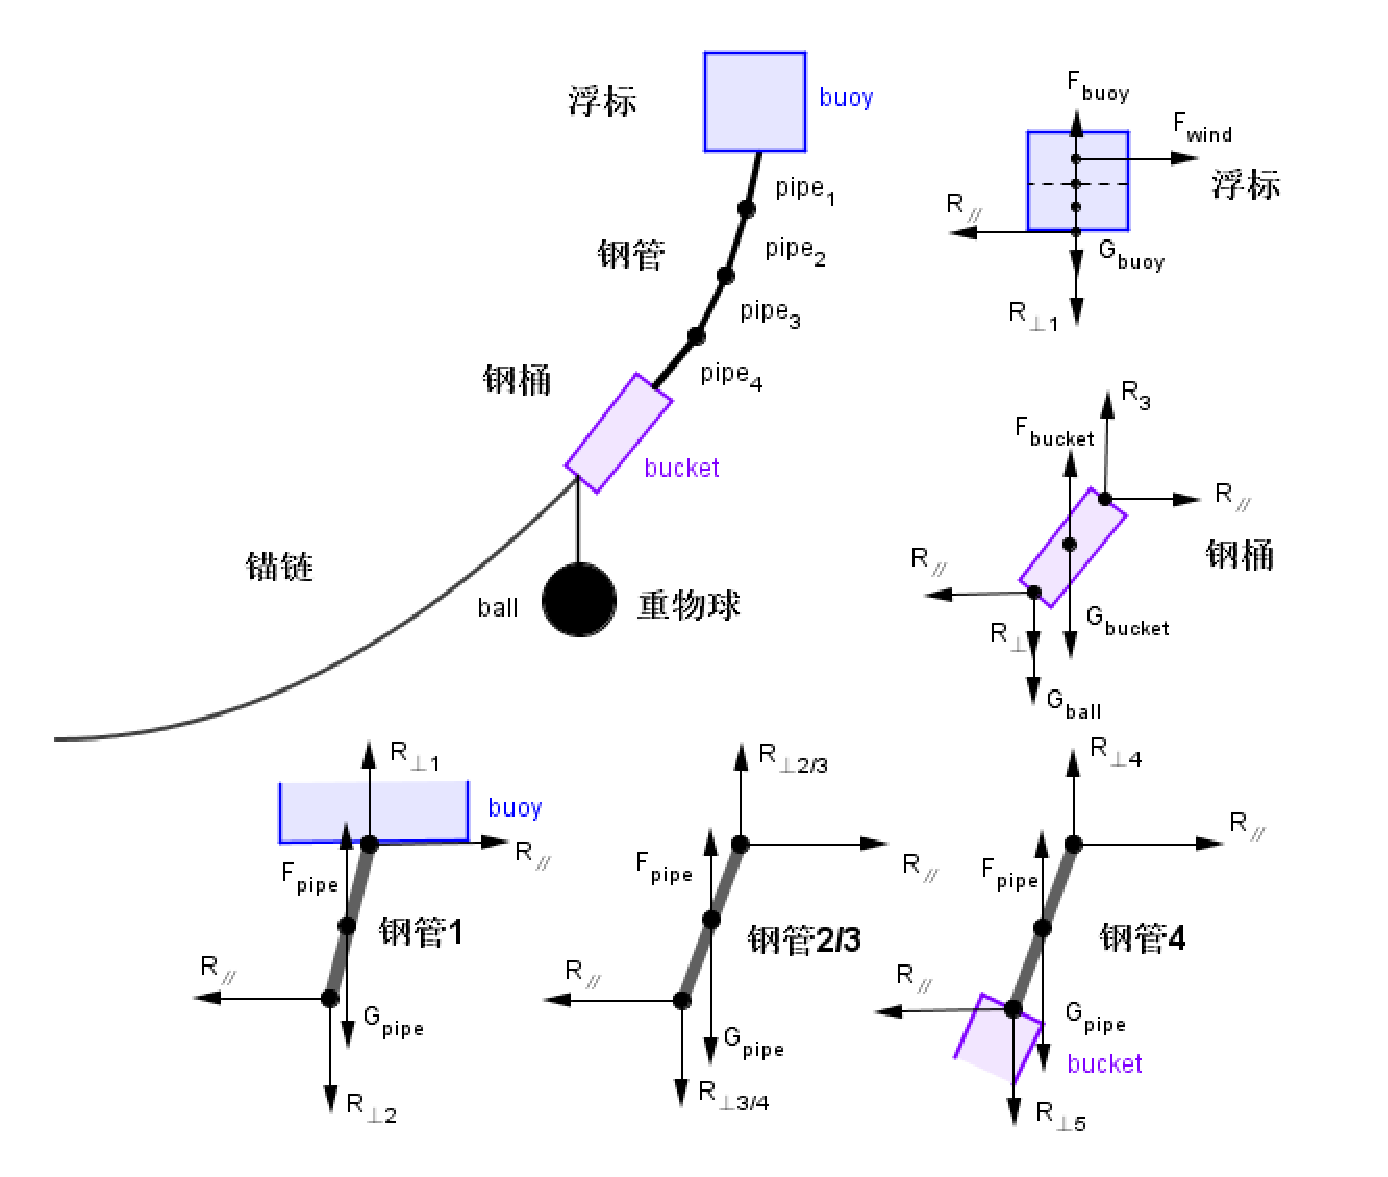
\includegraphics[width=400pt]{final.eps}1
\caption{模型及受力分析示意图}
\end{figure}

\begin{enumerate}
\item 每节链环长度相比于整条锚链非常小,故可作近似处理
\item 锚链主要用于连接锚和钢桶,本身体积小、浮力小,浮力可以忽略;重物球则用于调节钢桶的角度,且质量大,浮力效果不明显。
\item 对于此题而言,可以认为铰链是一种合理的连接方式。下图是铰链的示意图:

\begin{figure}[H]
\centering
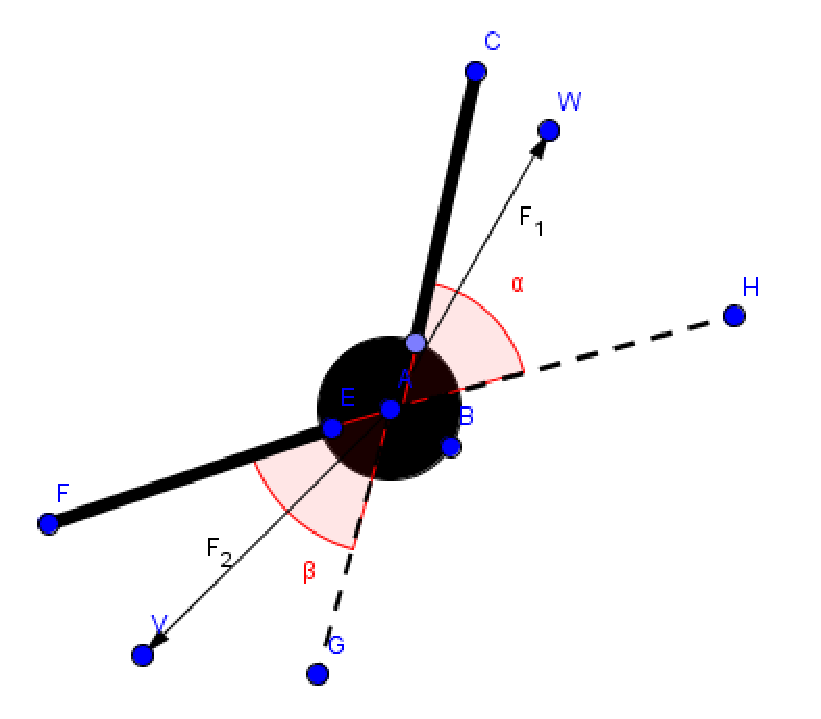
\includegraphics[width= 200pt]{1234.eps}
\caption{铰链}
\end{figure}

AC、AF分别为铰链的两臂,那么AC臂受铰链的力$F_2$反向延长线在$\angle\alpha$内,AC臂受铰链的力$F_2$反向延长线在$\angle\beta$ 内。
\item 为此,我们说明第1、2问在稳态时:必有$\theta_0>84.3^{\circ}$。\\
先讨论第一问:对于钢桶与钢管4的部分,若$\theta_5\ge\theta_4$,则如下图:\\

\begin{figure}[H]
\centering
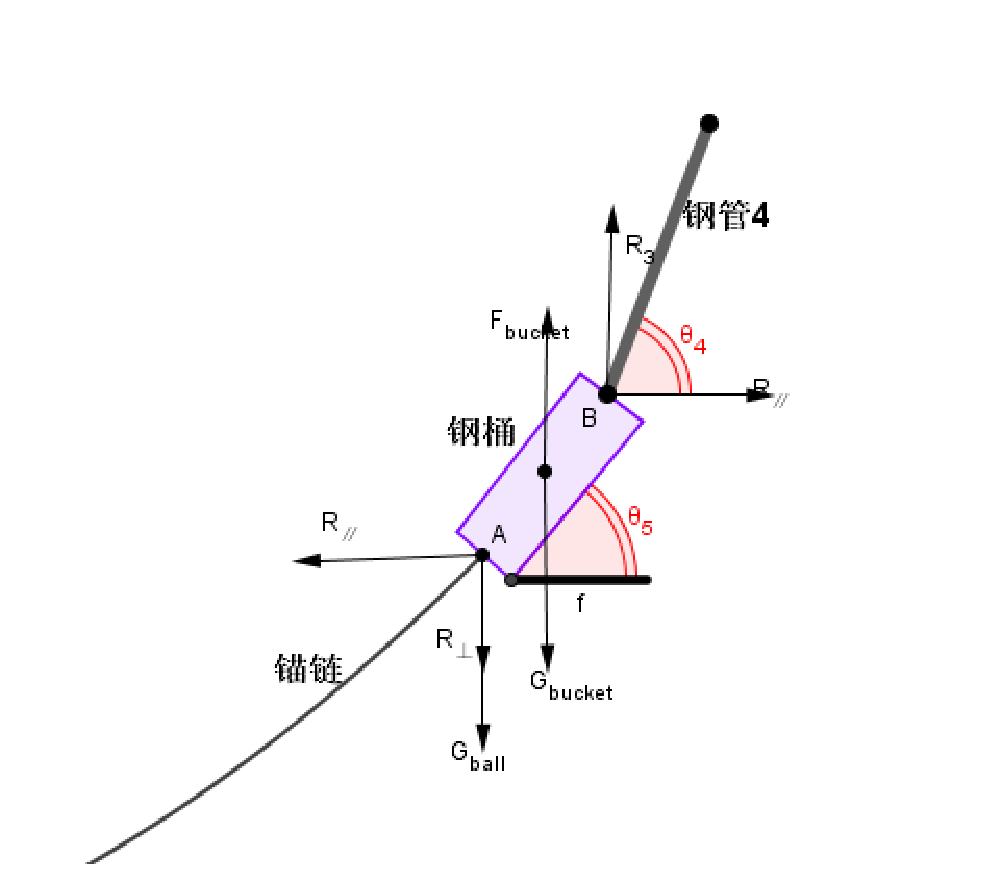
\includegraphics[width = 300pt]{123.eps}
\caption{钢管受力分析图}
\end{figure}

~~~~因悬链线对钢桶的力在竖直分量是向下的,故$R_{\perp5}+F_{bucket}<G_{bucket}$,从而$G_{bucket}-F_{bucket}>0$,又因钢管4对钢桶的力在$\angle \theta_4$内,于是对$A$ 点的力矩将会使钢桶顺时针转动,这与平衡态矛盾。故我们验证了$\theta_5<\theta_4$。

同理我们得到$\theta_5<\theta_4<\theta_3<\theta_2<\theta_1<\theta_0$,于是我们只需验证$\theta_5>84.3^{\circ}$即可。

由整体法不难知道,悬链线对B点的作用力在水平方向上的分量$R_{//}$方向为左、且该分量大小即$F_{wind}$.于是用符号$F_{wind}$去代替$R_{//}$.
对B点,由力矩平衡得到方程:\\
\begin{equation}
\frac{1}{2}(G_{bucket}-F_{bucket})cos(\theta_5)+(R_{\perp}+G_{ball})*cos(\theta_5)-F_{wind}sin(\theta_5)=0
\end{equation}
于是
\begin{equation}
\tan(\theta_5)=\frac{\frac{1}{2}(G_{bucket}-F_{bucket})+(R_{\perp}+G_{ball})}{F_{wind}}
\end{equation}
因$R_{\perp}>0, \ G_{bucket}=m_{bucket}g,\ F_{bucket}=\rho_wgh_3(\frac{d_3}{2})^2,\ G_{ball}=1200g, \ F_{wind}<0.625\times2(2-\Delta h)\times24^2$,取$v_风=24m/s$\\
代入数据得:
\begin{equation}
\tan(\theta_5)>\frac{12136.99}{720(2-\Delta h)}
\end{equation}
再对浮标受力分析知$F_{buoy}=\rho_w g\Delta h\pi (\frac{d1}{2})^2>G_{buoy}=m_{buoy}g$,解得
\begin{equation}
\Delta h>\frac{1}{0.9955202\pi}
\end{equation}
从而
$tan(\theta_5)>10.03235\rightarrow\theta_5>84.3077^{\circ}>84.3^{\circ}$。 于是$\theta_0>\theta_5>87^{\circ}$得证。由此我们可以知道,浮标在风速为24m/s时,与水平夹角已超过$87^{\circ}$(显然当风速为12m/s时,这一角度将会更大!)

~~~~再讨论第二问:由题目条件知:$\theta_5>85^{\circ}$,那么$\theta_0>\theta_5>84.3^{\circ}$,所以第一、二问总可以保证,$\theta_0>84.3^{\circ}$ 成立,计算知
$cos5.6^{\circ}= 0.9952274\approx1,sin5.6^{\circ}=0.0975829\approx0$
所以我们有理由把浮标当作与水面垂直来处理。

\item 从对称的角度来说,钢管与浮标的传输节点应为浮标底面圆的圆心,而由$4$的推导过程,第1节钢管和浮标均与海平面近似垂直,从而可以近似认为第1节钢管对浮标的约束力过浮标的重心。\\
\item 我们水流力和水平面有一定的倾斜角度,将水流力作水平、竖直上的分解,而竖直方向力对浮标将会很小。所以水流力可以近似水平。
\item 钢管密封可直接由钢管排水体积计算出钢管所受的浮力
\end{enumerate}

\subsection{模型1——力学模型(问题一\&问题二)}

~~~~问题1中需要确定各角度参量和锚链位形等几何参数,为此我们采用平面刚体静力学分析的方法对各传输节点进行受力分析,列出平衡状态方程组,并结合几何约束条件求解系统的各几何参数。

对一个由N个节点组成的平面刚体系统,若系统处于平衡状态,则对节点 $j$,其水平方向和竖直方向的合外力为零,取平面上任一点$O$ 为参考点,作用在节点$j$的各外力对$O$的合外力矩为零。即:
\begin{align}\label{PlanerRigidBodyEqulibriumEquation}
&\sum\limits_{k=1}^n F_{kx}  =0;\\
&\sum\limits_{k=1}^n F_{ky}  =0;\\
&\sum\limits_{k=1}^n F_{kx}r_kx+F_{ky}r_ky  =0;
\end{align}

上式(3)中$r_x$和$r_y$分别表示相应的力对$O$点的力臂。
利用上述模型,对各传输节点依次进行受力分析不难得出
\begin{equation}
R_{\parallel}=F_{wind}\label{MechanicsBegin}
\end{equation}
即各节点水平约束力相等,近海风$F_{wind}$可由下面的近似公式计算:
\begin{equation}
F_{wind}=0.625\times S v^2
\end{equation}
对于竖直方向上,有:
\begin{align}
&F_{buoy}=G_{buoy}+R_{\perp1}\\
&F_{pipe}+R_{\perp1}=G_{pipe}+R_{\perp2}\\
&F_{pipe}+R_{\perp2}=G_{pipe}+R_{\perp3}\\
&F_{pipe}+R_{\perp3}=G_{pipe}+R_{\perp4}\\
&F_{pipe}+R_{\perp4}=G_{pipe}+R_{\perp5}\\
&F_{bucket}+R_{\perp5}=G_{bucket}+G_{ball}+R_{\perp}
\end{align}
对于上述方程中出现的浮力项和重力项,我们有
\begin{align}
&F_{buoy}=\rho_w g \pi (\frac{d_1}{2})^2 \Delta h \\
&F_{pipe}=\rho_w g \pi (\frac{d_2}{2})^2 h_2 \\
&F_{bucket}=\rho_w g \pi (\frac{d_3}{2})^2 h_3 \\
&G_{buoy}=m_{buoy}g\\
&G_{pipe}=m_{pipe}g\\
&G_{bucket}=m_{bucket} g\\
&G_{ball}=m_{ball} g
\end{align}
取每个节点的圆柱底面中心为参考点,由力矩平衡可以得到:

\begin{align}
&(G_{pipe}-F_{pipe})\frac{h_2}{2}\cos(\theta_1)+R_{\parallel}h_2\sin(\theta_1)=R_{\perp1}h_2\cos(\theta_1)\\
&(G_{pipe}-F_{pipe})\frac{h_2}{2}\cos(\theta_2)+R_{\parallel}h_2\sin(\theta_2)=R_{\perp2}h_2\cos(\theta_2)\\
&(G_{pipe}-F_{pipe})\frac{h_2}{2}\cos(\theta_3)+R_{\parallel}h_2\sin(\theta_3)=R_{\perp3}h_2\cos(\theta_3)\\
&(G_{pipe}-F_{pipe})\frac{h_2}{2}\cos(\theta_4)+R_{\parallel}h_2\sin(\theta_4)=R_{\perp4}h_2\cos(\theta_4)\\
&(G_{bucket}-F_{bucket}) \frac{h_3}{2} \cos(\theta_5) + R_{\parallel} h_3 \sin(\theta_5) = R_{\perp5} h_3 \cos(\theta_5)	\label{MechanicsEnd}
\end{align}
\subsubsection{假设1--锚线全部长度被拉直}
根据文献\cite{catenery}中的分析,可以证明其几何位形为悬链线,$y=a\cosh(\frac{x}{a})$
其中
\begin{equation}
a=\frac{R_{\parallel}}{\rho_{cable}g} \label{GeometryBegin}
\end{equation}
\begin{figure}[H]
\centering
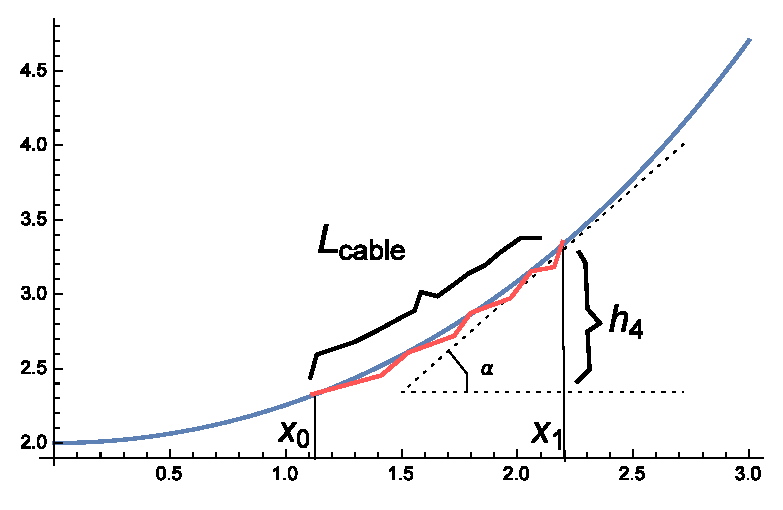
\includegraphics[scale=0.8]{MyCatenary.eps}
\caption{锚链形状}
\end{figure}

其相对$x=0$的弧长公式为$s=a\sinh(\frac{x}{a})$,而锚链为悬链线在$x>0$中$[x_0,x_1]$区间的曲线段,
即为上图中标为红色的曲线,由于钢筒与锚链间的约束力沿悬链线
在$x_1$处的切线,而切线倾角可通过对曲线方程求导得到,于是可得方程
\begin{equation}
\frac{R_{\perp}}{R_{\parallel}}=\sinh(\frac{x_1}{a})
\end{equation}
补充记号
\begin{tabular}{cc}
$L_{cable}$ & 锚链弧长  \\
$h_4$ & 锚链高度 \\
\end{tabular}
根据悬链线方程及其弧长公式可得:
\begin{align}
&h_4=a\cosh(\frac{x_1}{a})-a\cosh(\frac{x_0}{a})\\
&L_{cable}=a\sinh(\frac{x_1}{a})-a\sinh(\frac{x_0}{a})
\end{align}
此外,由总水深的几何约束条件可得:
\begin{equation}
h_w=\Delta h+h_2(\sin(\theta_1)+\sin(\theta_2)+\sin(\theta_3)+\sin(\theta_4))+h_3\sin(\theta_5)+h_4
\end{equation}
浮标在风向法平面的投影面积 \( S \)被下式给出:
\begin{equation}
S=d_1(h_1-\Delta h)  \label{GeometryEnd}
\end{equation}
上述(\ref{MechanicsBegin})-(\ref{MechanicsEnd})为力学关系方程式,(\ref{GeometryBegin})-(\ref{GeometryEnd})为几何关系方程式,共计26 个方程,
未知量有\\
\begin{center}
\begin{tabular}{ccc}
  \hline \hline
  % after \\: \hline or \cline{col1-col2} \cline{col3-col4} ...
参数类型 & 参数 & 数量\\ \hline
长度参量 & $\Delta h,h4,a,x_0,x_1$ &5\\
角度参量 & $\theta_1,\theta_2,\theta_3,\theta_4,\theta_5$ &5\\
浮力参量 & $F_{buoy},F_{pipe},F_{bucket}$ &3\\
重力参量 & $G_{buoy},G_{pipe},G_{bucket},G_{ball}$ &4\\
约束力参量 & $R_{\parallel},R_{\perp},R_{\perp1},R_{\perp2},R_{\perp3},R_{\perp4},R_{\perp5} $ & 7\\
其他参量 & $S,F_{wind}$&2\\
参数总计&&~~~~~~~26~~~~~~~~\\ \hline \hline
\end{tabular}
\end{center}
\subsubsection{假设2--锚线在锚点段有部分未被拉起}

~~~~在假设2下,如果方程仍然按照假设1中的形式,$x_0$和$\theta_6$可能出现负解,此时需重新设定原点,使锚链的方程改变,以消除负解的情况,这不仅是得到合理解的必要条件,也可以更准确地计算$L_{cable}$和$h_4$的值。

按照锚链的几何性质继续延长锚链与锚相连的一端(延长的部分在海床下面),直至某切线与海平面平行的点,将该点设为原点。其余各假定分析与模型1一致,那么(\ref{MechanicsBegin})-(\ref{GeometryEnd})这些方程中只改变了如下2个方程:\\
\begin{align}
&h_4=a(\cosh(\frac{x_1}{a})-1)\\
&L_{cable}=a\sinh(\frac{x_1}{a})
\end{align}

\subsubsection{模型的结果}

~~~~上面理论分析给出的含26个未知量的26个方程组成的方程组由于有三角函数项,可能存在多解,但对于符合现实情况的解,要满足如下的条件:

\begin{enumerate}
\item 所有未知量均为正数。
\item 所有角度参量均$\in[0,\frac{\pi}{2}]$。
\end{enumerate}

为了探究该方程组解的情况,我们采用消元的办法,将未知量的个数减为6,以下分别为假设1、假设2处理第一、二问的结果:(单位若未标出,则为国际标准单位)\\

\noindent \textbf{问题一:}

假设1

\begin{center}
\begin{tabular}{ccc}
\hline \hline
\multicolumn{1}{c}{参数}&\multicolumn{1}{c}{$v_w=12m/s$}&\multicolumn{1}{c}{$v_w=24m/s$}\\
\hline
$\theta_1$ & $89.0379^{\circ}$& $86.2641^{\circ}$\\
$\theta_2$ & $89.0323^{\circ}$&$86.2429^{\circ}$\\
$\theta_3$ & $89.0266^{\circ}$& $86.2214^{\circ}$\\
$\theta_4$ & $89.0209^{\circ}$& $86.1996^{\circ}$\\
$\theta_5$ & $89.0079^{\circ}$&$86.1503^{\circ}$\\
$a$ & $3.306$ & $13.1307$\\
$x_1$&$7.8387$&$16.7818$\\
$x_0$&$-3.6915$&$-0.3115$\\
$\theta_6$&$-53.7377$&$-1.3591$\\
$\delta h$&$0.7389$&$0.7489$\\
$R_{move}$&$12.153$&$18.4233$\\ \hline \hline
\end{tabular}\\
\end{center}
假设1中$x_0$和$\theta_6$均出现负值,不符合非负的假定。分析其物理原因,可能是锚线靠近锚点端存在未被拉起的部分,即假设2.\\

假设2

\begin{center}
\begin{tabular}{ccc}
\hline \hline
\multicolumn{1}{c}{参数}&\multicolumn{1}{c}{$v_w=12m/s$}&\multicolumn{1}{c}{$v_w=24m/s$}\\
\hline
$\theta_1$ & $89.0226^{\circ}$& $86.2640^{\circ}$\\
$\theta_2$ & $89.0168^{\circ}$& $86.2428^{\circ}$\\
$\theta_3$ & $89.0110^{\circ}$& $86.2213^{\circ}$\\
$\theta_4$ & $89.0051^{\circ}$& $86.1995^{\circ}$\\
$\theta_5$ & $88.9917^{\circ}$& $86.1502^{\circ}$\\
$a$ & $3.3198$ & $13.1308$ \\
$x_1$&$7.3967$&$16.7797$ \\
$x_0$&$0$&$0$ \\
$\theta_6$ & $0$ & $0$ \\
$\delta h$&$0.7348$&$0.7489$\\
$R_{move}$&$8.4832$&$18.1097$ \\
\hline \hline
\end{tabular}\\
\end{center}
此时各项系数均正,符合题意。\\
于是我们根据假设2作出风速=12m/s和风速=24m/s锚线的形状图像(内附显式表达)\\
\begin{figure}[H]
\centering
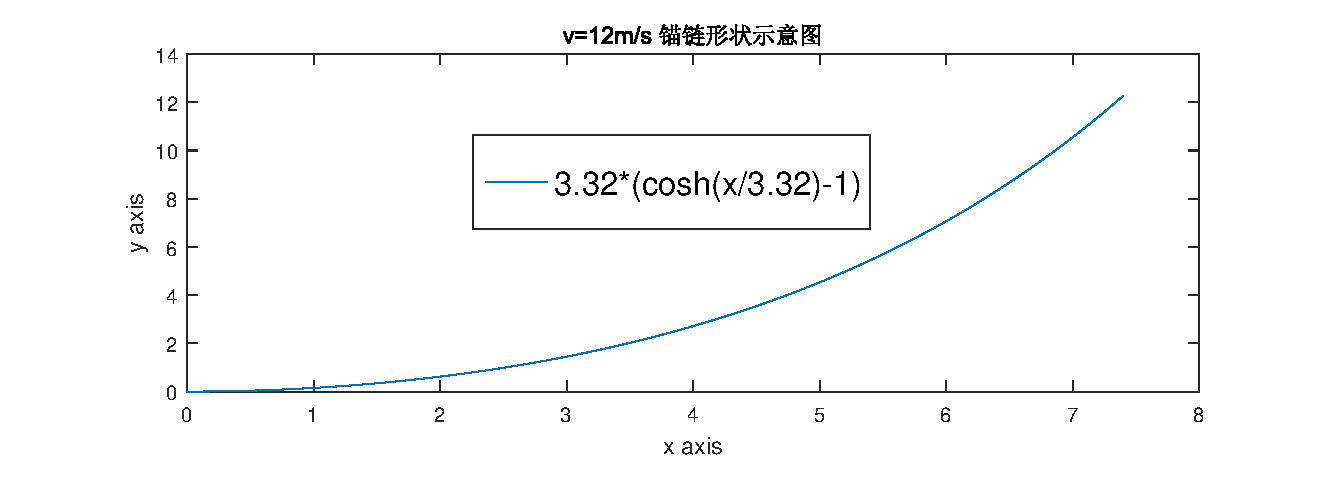
\includegraphics[width=380pt]{V12ms.eps}
\caption{风速=12m/s时锚线形状}
\end{figure}

\begin{figure}[H]
\centering
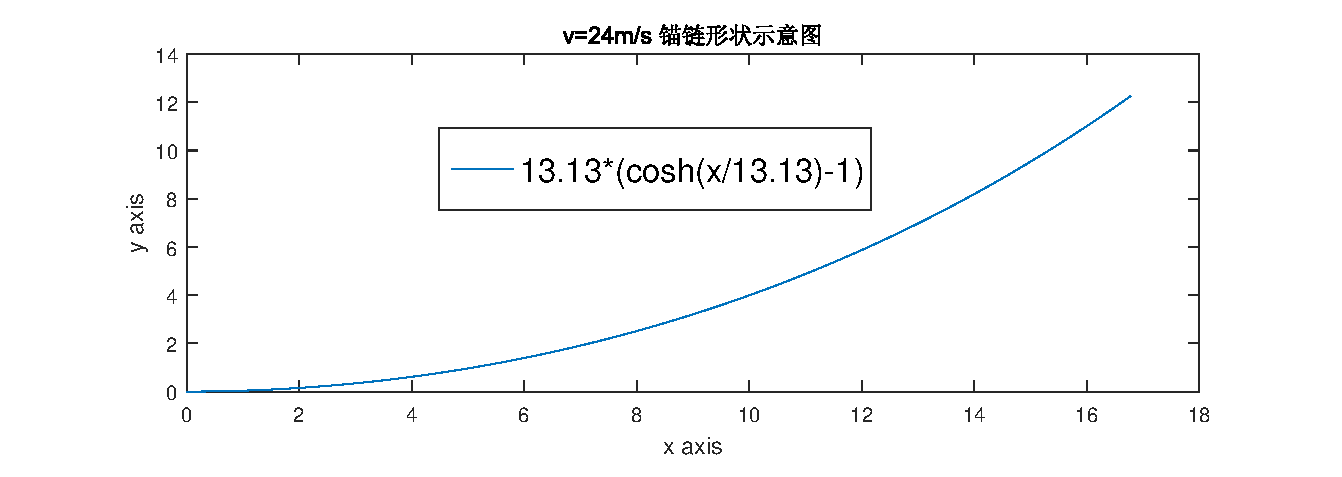
\includegraphics[width=380pt]{V24ms.eps}
\caption{风速=24m/s时锚线形状}
\end{figure}


\noindent \textbf{问题二:}

假设2\\
\begin{center}
\begin{tabular}{ccc}
\hline \hline
\multicolumn{1}{c}{参数}&\multicolumn{1}{c}{$v_w=36m/s$}\\
\hline
$\theta_1$ & $82.1546^{\circ}$\\
$\theta_2$ & $82.1124^{\circ}$\\
$\theta_3$ & $82.0698^{\circ}$\\
$\theta_4$ & $82.0267^{\circ}$\\
$\theta_5$ & $81.9292^{\circ}$\\
$a$ & $29.0460 $ \\
$x_1$&$27.2596$ \\
$x_0$&$9.2348$ \\
$\theta_6$ & $17.9107$  \\
$\delta h$&$0.7700$\\
$R_{move}$&$19.7156$ \\
\hline \hline
\end{tabular}
\end{center}

各项数据都很合理,于是我们作出风速=36m/s锚线的形状图像\\

\begin{figure}[H]
\centering
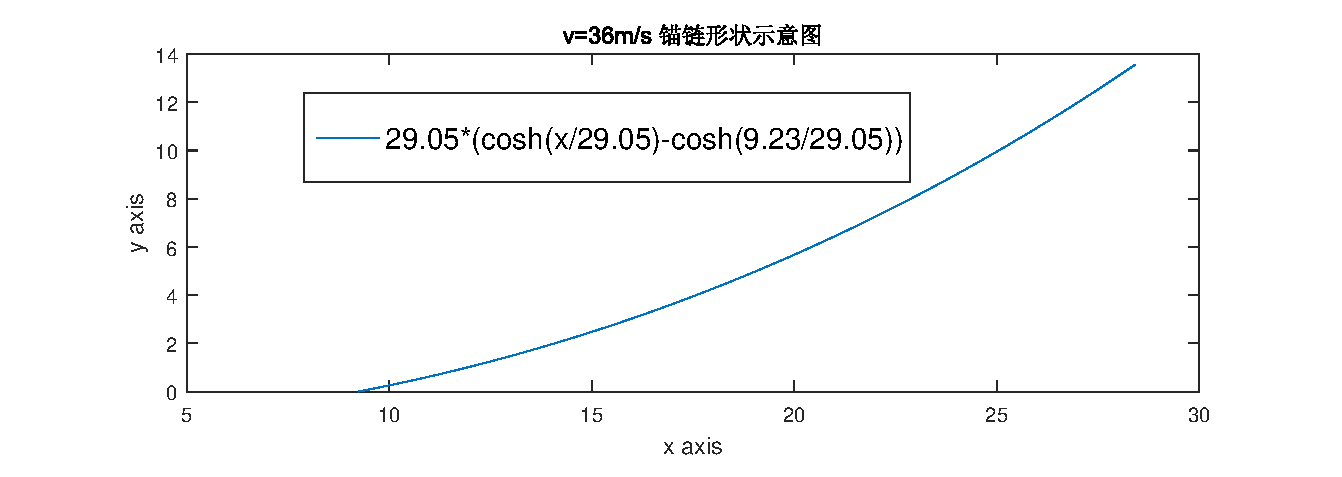
\includegraphics[width=380pt]{V36ms.eps}
\caption{风速=36m/s时锚线形状}
\end{figure}

接着我们给出随着重物球质量变化,两个角度的变化趋势如下图:\\

\begin{figure}[H]
\centering
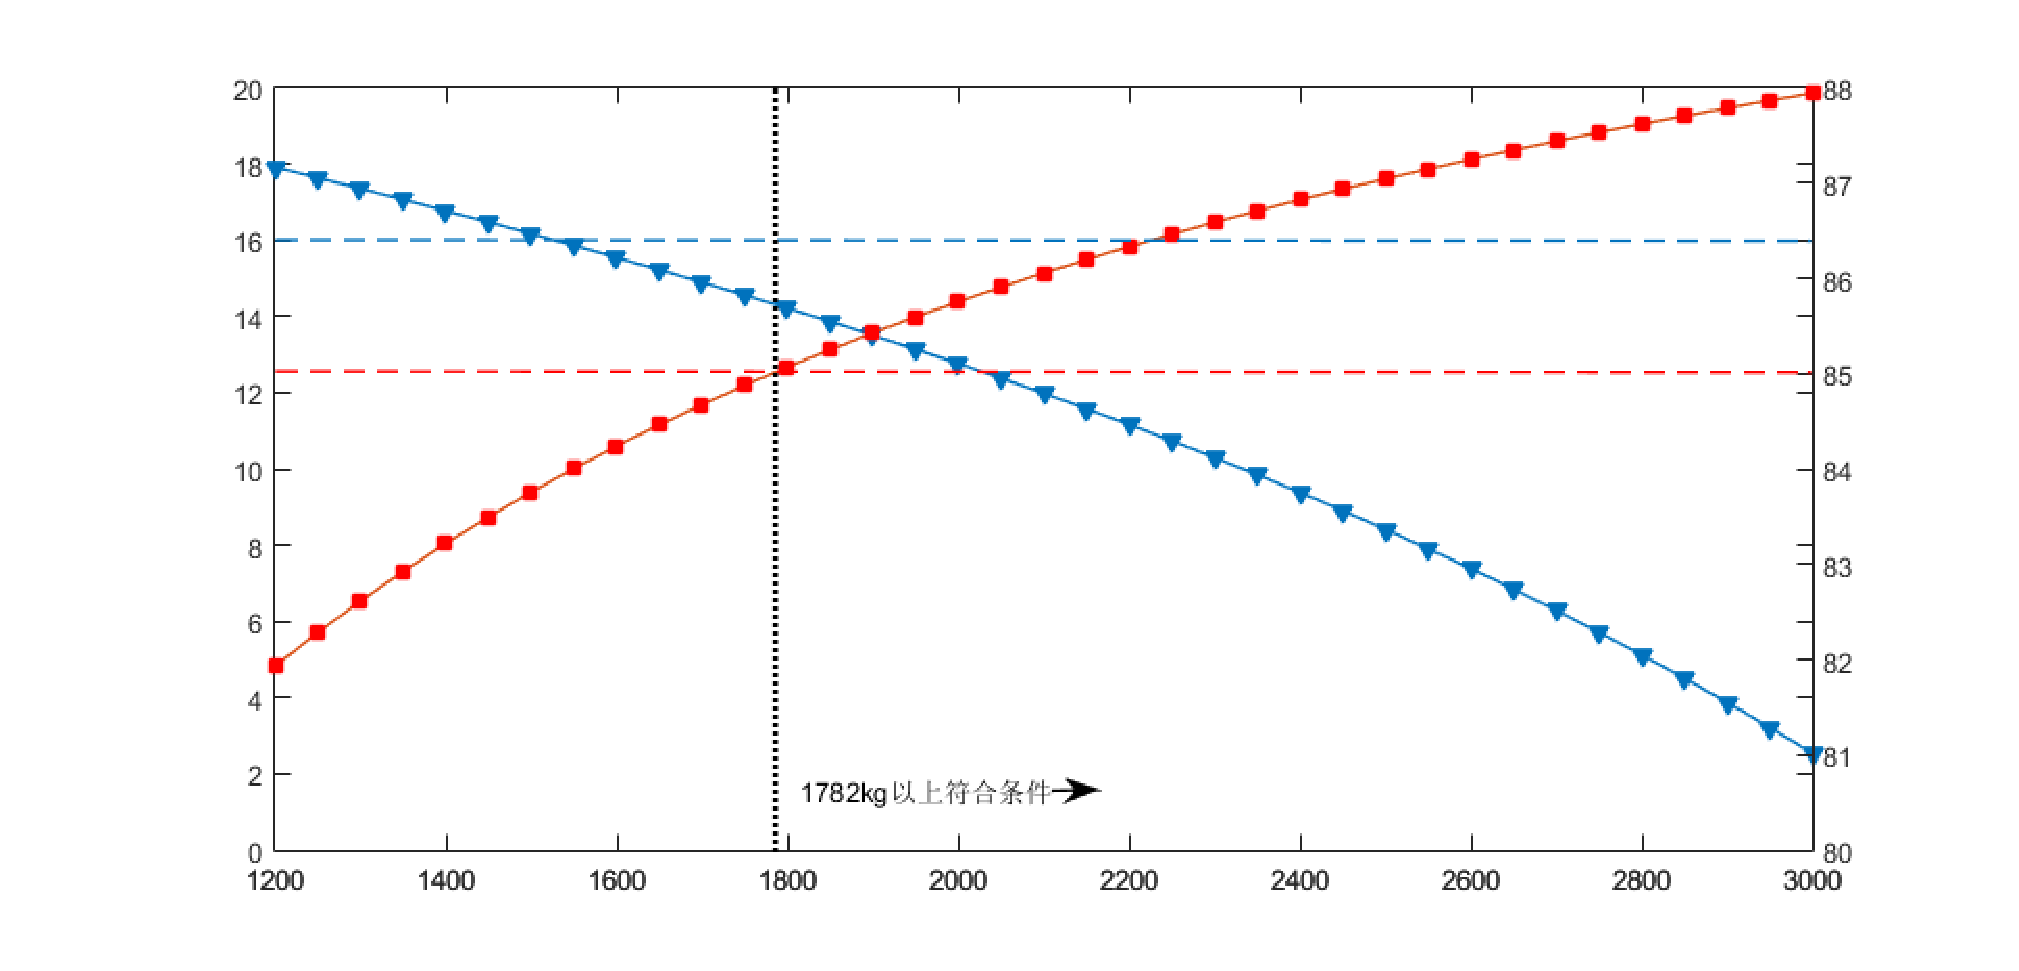
\includegraphics[width = 380pt]{question2.eps}
\caption{重物球质量-两个角度变化}
\end{figure}

\begin{figure}[H]
\centering
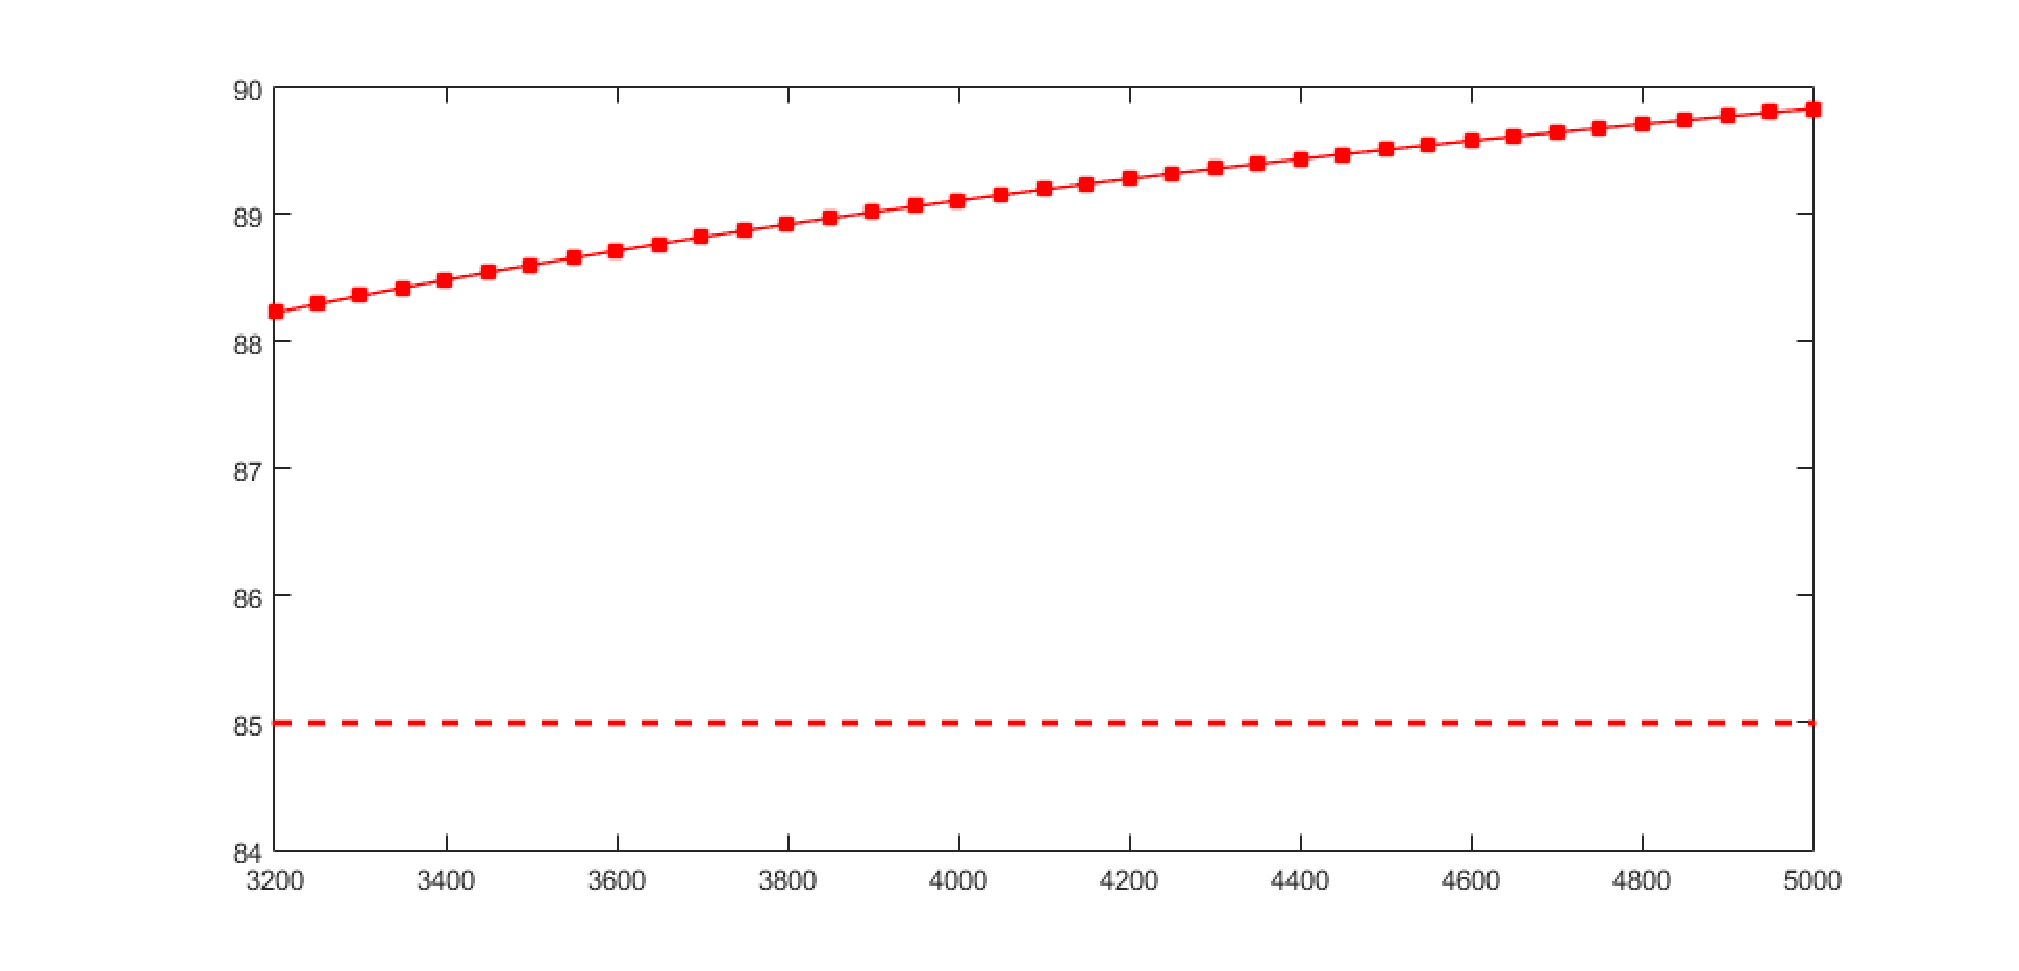
\includegraphics[width=380pt]{question2_2.eps}
\caption{重物球质量较大时对钢桶角度的影响}
\end{figure}

 由趋势图可见随着重物球质量$G_{ball}$的增加,钢桶与水平方向的夹角$\theta_5$增加,锚链与海床的夹角$\theta_6$减小。
 特别的,当$\theta_5=1782kg$时,两种角度都达标,而当$\theta_5=5304kg$时,浮标完全浸没水中。所以我们认为$[1782kg,5304kg]$ 为重物球质量$\theta_5$合适的区间。\\

 以下附两张表可以看出$\theta_5$取特定值时两个角度具体变化:

\begin{center}
\begin{tabular}{cccccc}
\hline \hline
重物球质量($m_{ball}$/kg) & 1200  &  1600  &  2000  &  2400  &  2800 \\ \hline
钢桶圆柱与水平方向的夹角($\theta_5 /^{\circ}$)&81.9292 &  84.2387 &  85.7539  & 86.8228  & 87.6168 \\
锚链与海床的夹角($\theta_6/^{\circ})$)&17.9170  & 15.5411 &  12.7628 &   9.3822 &   5.1235\\
\hline \hline
\end{tabular}
\end{center}


\begin{center}
\begin{tabular}{cccccc}
\hline \hline
重物球质量(kg) & 3200  &  3600  &  4000  &  4400  &  4800 \\ \hline
钢桶圆柱与水平方向的夹角($\theta_5 /^{\circ}$)&88.2298 &  88.7164 &  89.1112 &  89.4378 &  89.7120 \\
锚链与海床的夹角($\theta_6/^{\circ})$)&0&0&0&0&0\\
\hline \hline
\end{tabular}
\end{center}


\subsection{模型2——力学模型+罚函数模型(问题三)}
\subsubsection{模型的建立与分析}

~~~~设变量$N$是锚链型号,$L_{cable}$是长度,$m_{ball}$是重物球的质量。

状态量$F_{wind}$是风力大小,$F_{flow}$是水流力大小,$angle$是风力水流力夹角大小,$h_{w}$是水深高度。因为假设浮标是垂直的,计算时不考虑风力与水流力对浮标倾斜的影响,为了方便计算,我们使用由风力、水流力组成的合力来计算,这样就可以套用之前的模型。考虑系泊系统要求浮标的吃水深度,游动区域和钢桶的倾斜角度尽可能小。我们从这个角度构造如下惩罚函数
\[F(N,L_{cable},m_{ball},F_{wind},F_{flow},angle,h_{w})\]
\[=max\{\theta_{6}-16,0\}+(\frac{R_{move}}{30})^2+(\frac{90-\theta_{5}}{5})^2+(\frac{\Delta h}{h_{w}})^2=F\]\\
注:

1.在\(N,L_{cable},m_{ball},F_{wind},F_{flow},angle,h_{w}\)给定时,\(\Delta h,R_{move}\,\theta_{5},\theta_{6}\) 可由模型1解出,故\[max\{\theta_{6}-16,0\}+(\frac{R_{move}}{30})^2+(\frac{90-\theta_{5}}{5})^2+(\frac{\Delta h}{h_{w}})^2\]
可看成\(N,L_{cable},m_{ball},F_{wind},F_{flow},angle,h_{w}\)的函数。上式的合理性得以证明。
\\

2.$\theta_{6}>16^o$,说明锚被拖行,惩罚因子大于0。第二项代表游动区域的惩罚项,游动区域的半径有上界30米,故此惩罚项数值不大于1,半径越小,惩罚越小。第三项是钢桶倾斜角的惩罚项,如果钢桶不倾斜的时候,无惩罚,钢桶倾斜超过$5^o$时,惩罚数值大于1,倾斜程度越大,惩罚数值越大,超过$5^o$增长速度很快。第四项是吃水深度的惩罚项,很明显,吃水越深,惩罚越大,此惩罚项数值不大于1。 因为锚链与海床夹角超过$16^o$ 时锚会被拉起,造成浮标位置的丢失,这是绝对不能出现的情况。所以这个惩罚系数比较大;钢桶的倾斜角度会影响设备工作质量,所以惩罚系数相对较大;游动区域和吃水深度对于设备工作无影响,只是可能会影响浮标位置的精确程度,所以它们的惩罚函数相对来说较小。\\

3.{\color{red}{函数内部逻辑}}

   step1:先用模型1中的假定2判断绳是否被拉直,若是(Truth1),再用$fsolve$函数判断其是否有解,若有解,则代入F计算,不然舍去。

   step2:在step1的第一步逻辑判断为否(False1):判断$\delta h$和$L_{cable}$是否在相应的可能区间内,若是(truth2),再用第一项表示锚链与海床的夹角的惩罚项,如果角度$\theta_{6}\leq 16^o$,说明锚不会被拖行,满足题目,不设惩罚;如果$fsolve$函数判断其是否有解,若有解,则代入F计算,不然舍去

   step3:在step2的第二步逻辑判断为否(False2);令 F$=4$ .这里4也是经过我们反复计算得到的合理判断值\\

\subsubsection{模型的结果}

~~~~经过一些极端数据和一般数据测试,我们发现对于第一项数值很大,后三项的惩罚项数值比较小,符合我们的初始预期,所以我们认为这个惩罚函数是合理的。

	然后我们假设四个状态量分布为均匀分布,对四个状态量随机变量进行均匀的取点,得到1260组状态,假设所有状态出现的概率相等。我们认为这些状态的惩罚函数之和
\[Sum(N,L_{cable},m_{ball})=\sum_{i,j,k,t} F(N,L_{cable},m_{ball},F_{wind,i},F_{flow,j},angle_{k},h_{w,t})\]
最小时,相应的$N,L_{cable},m_{ball}$是对所有状态来说最优的解。

在求使得惩罚函数之和$Sum$最小的解($N^*$,$L_{cable}^*$,$m_{ball}^*$)这些状态量时,注意到$N$是离散量,应对$N$进行枚举。对于每个$N$,理论上我们可以用F关于$L_{cable}$,$m_{ball}$的Hessian Matrix来求出其极小值,但是实际操作中因为需要用锚链长度$L_{cable}$,球的重量$m_{ball}$来表示惩罚函数的一些参数,这种计算方法在求导时计算量及其庞大,所以我们先用$L_{cable}$,$m_{ball}$ 的离散的步长进行枚举。此方法得到第五种锚链是最佳材料。

\begin{center}
\begin{table}[!ht]
\begin{tabular}{ccccccccc}
  \hline \hline
  % after \\: \hline or \cline{col1-col2} \cline{col3-col4} ...
锚链长度(m)	&	16	&	18	&	{\color{red}{20}}	&	22	&	24	&	26	&	28	&	30	\\ \hline
型号1	&	23.0379	&	14.3108	&	8.7168	&	5.1245	&	2.9698	&	1.8157	&	1.3138	&	1.1658	\\
型号2	&	16.0174	&	7.6547	&	3.4385	&	1.5768	&	0.9544	&	0.8336	&	0.8338	&	0.8473	\\
型号3	&	9.8131	&	3.303	&	1.1518	&	0.7009	&	0.659	&	0.6627	&	0.6647	&	0.6652	\\
型号4	&	5.5636	&	1.329	&	0.6175	&	0.5739	&	0.5755	&	0.5758	&	0.5758	&	0.5758	\\
{\color{red}{型号5}}	&	2.9843	&	0.6721	&	{\color{red}{0.5286}} 	&	0.5295	&	0.5296	&	0.5296	&	0.5296	&	0.5296	\\
  \hline \hline
\end{tabular}
 \caption{重物球质量为$2400kg$时惩罚函数的值}
\end{table}
\end{center}

因为锚链型号为\uppercase\expandafter{\romannumeral4},\uppercase\expandafter{\romannumeral5} 的材料密度差距有百分之十以上,几乎可以确定步长对材料选择的影响比较小。我们将$m_{ball}$固定,取这一截面的数据,发现型号\uppercase\expandafter{\romannumeral4}的惩罚数值总比\uppercase\expandafter{\romannumeral5}的大。特别的,取$m_{ball}=2400$的截面 如上表所示,故上述猜想是合理的。

在确定,第五种锚链材料是最优材料后,然后再将$L_{cable}$ 的步长缩小,求更精确使得惩罚函数最小的$L_{cable}$ 的值。对于$m_{ball}$,我们之前计算时考虑步长为200kg,由于考虑到实际情况,重物球的质量应该都是一百的倍数,故误差不大,就不再进行细分,沿用之前求出的结果。

\begin{figure}
  \centering
  % Requires \usepackage{graphicx}
  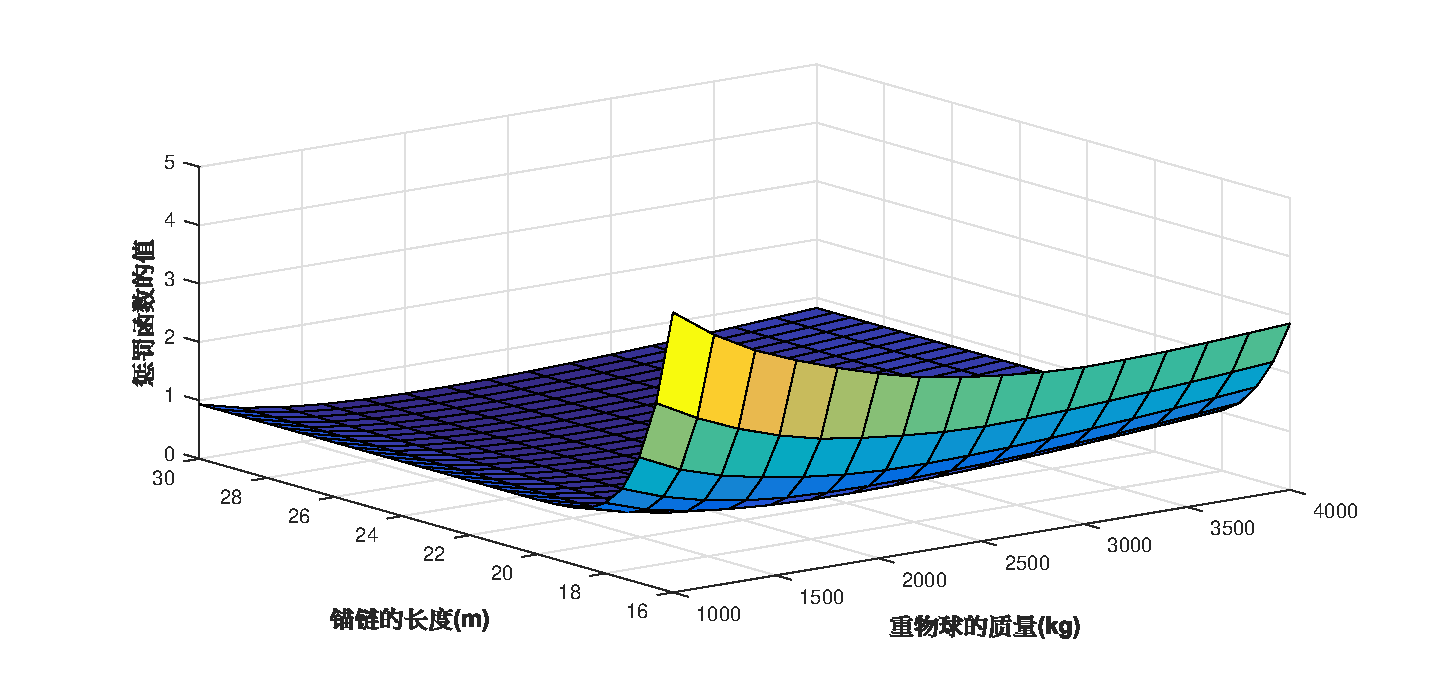
\includegraphics[scale=0.6]{question3_1.eps}
  \caption{材料\uppercase\expandafter{\romannumeral5}惩罚函数}\label{}
\end{figure}

计算可知惩罚函数最小值为0.5286,此时$L_{cable}=20,m_{ball}=2400$,即,链长20米,约111根材料\uppercase\expandafter{\romannumeral5},重物球的质量为2400kg。 惩罚函数与链长和重物球质量图像如图7所示。



\section{一些改进的模型}

针对第一、二题,以下模型提供了新的思路。(精确的解答还是参见之前的模型,以下模型仅供参考)\\
\begin{figure}[H]
\centering
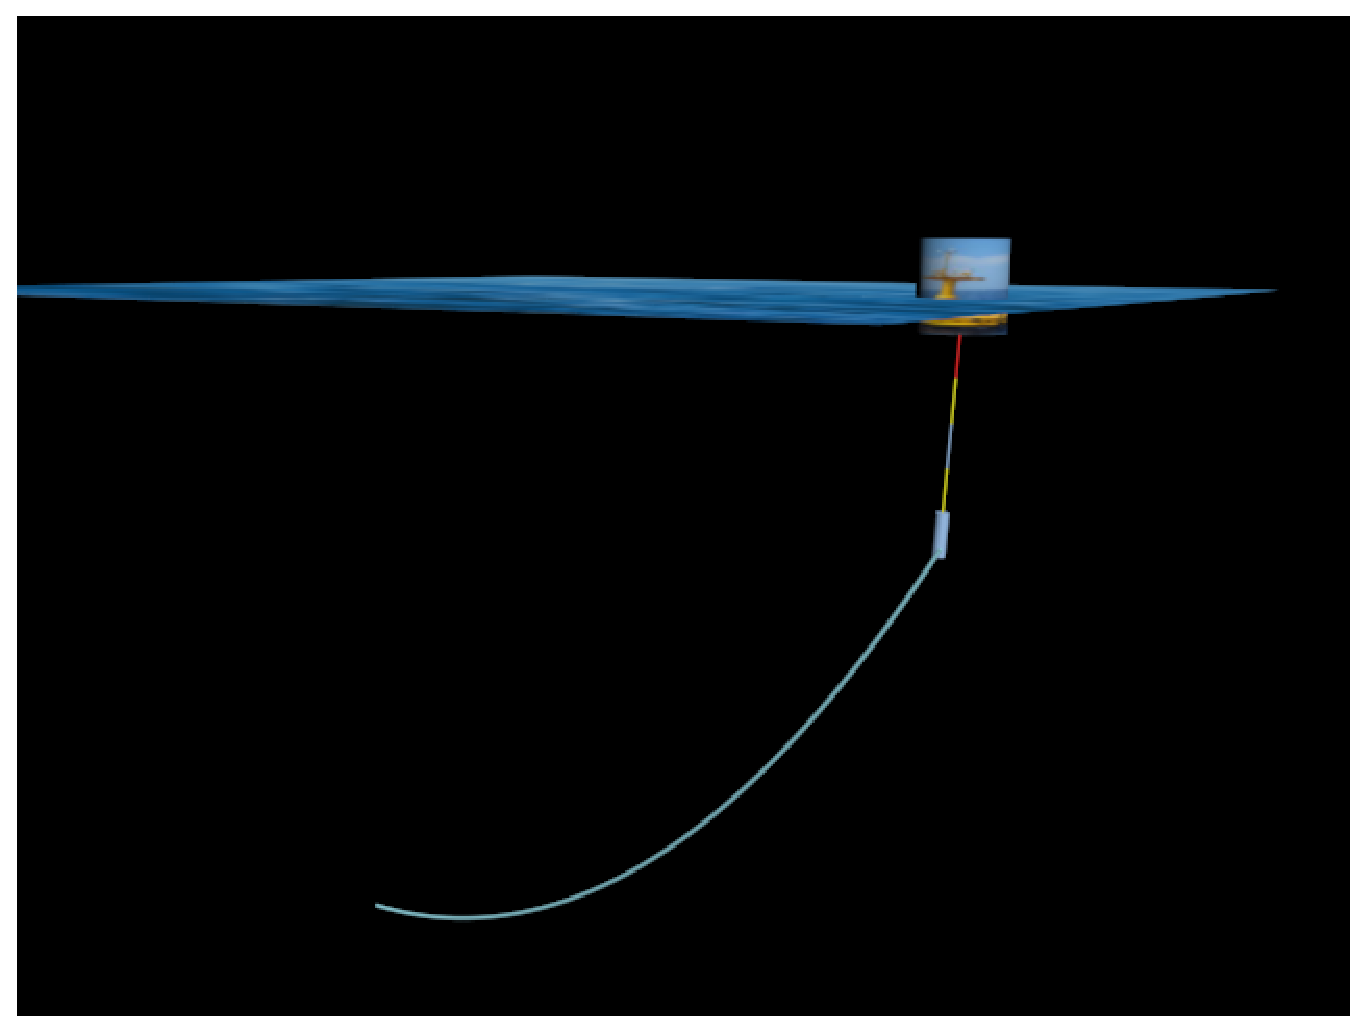
\includegraphics[width=400pt]{system.eps}1
\caption{建模小组成员自制系锚系统示意图(3D)}
\end{figure}
\subsection{模型3——能量模型}
\subsubsection{模型分析}
本系统由可近似成连续介质的锚链和若干可当成整体考虑的刚性圆柱体组成,认为其相互之间均为铰接,为一保守系统,可以采用能量的观点并从变分的角度推导出本系统各待求几何位形参量所满足的方程。
\subsubsection{模型建立}
对于一保守系统,自由度为N,广义坐标$\overrightarrow{q}=(q_1,q_2,...q_N)$,取定参考点$O$,对于作用在系统各节点的广义保守力,其对应一势函数
$\phi(\overrightarrow{q})=-\int_O^{\overrightarrow{P}} \overrightarrow{F}(\overrightarrow{q})\,dx$,其中$\overrightarrow{P}$为广义力$\overrightarrow{F}$的作用点,
系统的广义势函数为各广义力的势函数之和。
这种方法即是采用Lagrange力学求解平衡问题,此时本系统的Lagrangian 仅由势能项组成:$L=V(q_1,q_2,...q_N)$。系统的平衡状态的必要条件为$\frac{\partial V}{\partial q_i}=0,i=1,...N.$
上述方法可以推广到连续介质的无穷维系统,此时需要以连续体的位形函数$q(x)$代替单自由度的$q_1$,以对$q(x)$取变分代替对$q_1$的求导。
本题所描述的系统为一连续介质与可看成离散的节点的若干圆柱的混合,仍可采用上述方法进行分析。各节点所受的浮力、重力和浮标所受的风力均可看作广义保守力,取锚链末端为参考点$O$,建立平面直角坐标系,以$y(x)$描述锚链的方程,锚链末端点$(x_{end},y(x_{end}))$则锚链的重力势能为
\begin{equation}\label{StartGeneralPotential}
E_{Gcable}=\rho_{cable}g \int_0^{x_{end}} y\sqrt{1+y'^2}\,dx
\end{equation}
除$y(x)$外,系统的广义坐标还有$x_{end},\theta_1$至$\theta_5$以及浮标入水的深度$\Delta h$.
对于各圆柱体节点,不难写出其重力势能与浮力对应的广义势能之和为:
\begin{multline}
E_{\perp cylinder}=G_{ball} y(x_{end})+(G_{bucket}-F_{bucket})(y(x_{end})+\frac{h_3}{2}\sin(\theta_5))\\
+(G_{pipe}-F_{pipe})\sum_{i=1}^4 \lbrace y(x_{end})+h_3 \sin(\theta_5)+\sum_{j=1}^{i-1} (h_2 \sin(\theta_j)+\frac{h_2}{2} \sin(\theta_i))\rbrace
+(G_{buoy}-F_{buoy})(h_w-\Delta h +\frac{h_1}{2})
\end{multline}
风力只作用在浮标上,其广义势为:
\begin{equation}\label{EndGeneralPotential}
E_{wind}=-F_{wind}(x_{end}+h_3 \cos(\theta 5)+\sum_{i=1}^4 h_2 \cos(\theta_i)
\end{equation}
上述(\ref{StartGeneralPotential})-(\ref{EndGeneralPotential})相加即得系统广义势函数。但考虑到各广义坐标之间并不完全独立,还要满足水深约束和链长约束:
\begin{align}\label{WaterDepthConstraint}
&h_w=\Delta h+h_2(\sin(\theta_1)+\sin(\theta_2)+\sin(\theta_3)+\sin(\theta_4))+h_3\sin(\theta_5)+y(x_{end}) \\
&L_{cable}=\int_0^{x_{end}} \sqrt{1+y'^2}\,dx
\end{align}
至此,求解系统平衡位形的问题可陈述为在满足上述两种约束的条件下使系统广义势函数取得极小值。
\subsubsection{模型的求解}
对于上述带等式约束的优化问题,可采用Lagrange乘子法来求解。根据文献\cite{CalculusVariation}关于等周问题的讨论,对于无限维的锚链该方法也适用,取$\lambda_1,\lambda_2$为乘子,只需求如下函数的无约束极值:
\begin{multline}
E_{unconstrained}=E_{\perp cylinder}+E_{wind}
+\lambda_1 (h_w-\Delta h-h_2 \sum_{i=1}^4 (\sin(\theta_i))-h_3\sin(\theta_5)-y(x_{end}))\\
+\rho_{cable}g \int_0^{x_{end}} (y+\lambda_2)\sqrt{1+y'^2}\,dx -\lambda_2 L_{cable}
\end{multline}
对于上式,通过对$x_{end},\theta_1..\theta_5,\Delta h$求导不难得到含$\lambda_1,\lambda_2,y'(x_{end})$的方程。
而对于自由变量$y(x)$,其边界条件为左端点$O$固定,但右端点可移动,上式对$y(x)$取变分$\delta(y)$,并利用分部积分
公式可得:
\begin{equation}
\int_0^{x_{end}} (\frac{\partial f}{\partial y}- \frac{d}{dx}(\frac{\partial f}{\partial y'}))\delta y\,dx
+((\frac{\partial f}{\partial y'}y')_{x=x_{end}}-(G_{ball}+G_{buc}-F_{buc}+4(G_p-F_p)-\lambda_1))\delta y_{|x=x_{end}}
\end{equation}
上式$\delta y$与$\delta y_{|x=x_{end}}$前面的系数应为零,对于前一式,根据文献\cite{CalculusVariationOfCatenary}可以求出其通解,利用其端点值及长度已知的条件可得包含链条曲线系数在内的非线性方程组。通过与模型1的对比我们发现:
$\lambda_1=F_{buoy}-G_{buoy}$,$(G_{ball}+G_{buc}-F_{buc}+4(G_p-F_p)-\lambda_1$表示$R_{\perp}$,而$\delta y_{|x=x_{end}}$的系数即表示锚链与钢桶竖直方向相互作用力大小相等,我们通过与模型一的对比进一步证明了由此种方法得到的方程组与模型1等价,但限于篇幅证明过程此处略去。尽管模型二的推导并不直观,但如果能设计出从数值上极小化$E_{unconstrained}$的迭代算法,那么模型二的陈述是有意义的。但很可惜,由于$E_{unconstrained}$同时包含无穷维的函数
$y(x)$和等式约束,我们暂时无法给出直接求广义势函数极小值点的算法。
\subsubsection{模型的检验}
在模型1的数值求解中,我们给出了基于Matlab的fsolve的方法,下面我们在Mathematica中用自己设计的二分法求解描述该系统的非线性方程组。\\

由(26)及(27)式可解出$x_0,x_1$:
\begin{align}
& arcsinh (\sqrt{\frac{L_{cable}^2-h_4^2}{4a^2}})=\frac{x1-x0}{2a};\\
& arccosh (\frac{L_{cable}^2+h_4^2}{L_{cable}^2-h_4^2})=\frac{x0+x1}{a};
\end{align}
上两式为关于$x_0,x_1$的线性方程组,可解出$x_0,x_1$;

由(6)至(11)式可解出各约束力,将其代入(19)至(23)式,从而各角度的正切值也可表式出,具体推导过程由于篇幅所限放到了附件中。通过消元最终可得到关于
$\Delta h$的隐式方程,该隐式方程也考虑到了$x_0>0$的约束,若该条件不满足,则自动视锚链没有完全拉直,
具体可参考“NonLinearSolver.nb”文件中定义为SolverFunction函数,通过二分法的求解程序
NonLinearSolver($x_{left}$,$x_{right}$,iterativeTime)可得到$\Delta h$的数值解。
我们用该算法的数值结果与模型一中用fsolver的结果相同。

\subsection{模型4——考虑浮标的倾斜角度}
\subsubsection{模型分析}
在模型1、2的分析中,均将作用在浮标上的力视为共点力,浮标始终竖直向上,但实际情况是浮标可能会有倾斜,下面我们将浮标考虑在内,设浮标倾斜角为$\theta_0$,浮标浸水深度定义为浸水最底点到水面的距离。在模型2的求解中,我们推导出了$\Delta h>0.70$的条件
(具体见“NonLinearSolver.nb”文件),而由之前的讨论可知浮标倾角接近$90^{\circ}$,故水面应与浮标圆柱的\textbf{侧面}相交而钢筒不会露出水面。
\subsubsection{模型建立}
下图展示了浮标倾斜时的剖面图,按照浮标剖面矩形的长和宽的方向建立$z-x$坐标系,
\begin{figure}[!ht]
\caption{浮标倾斜剖面图}
\centering
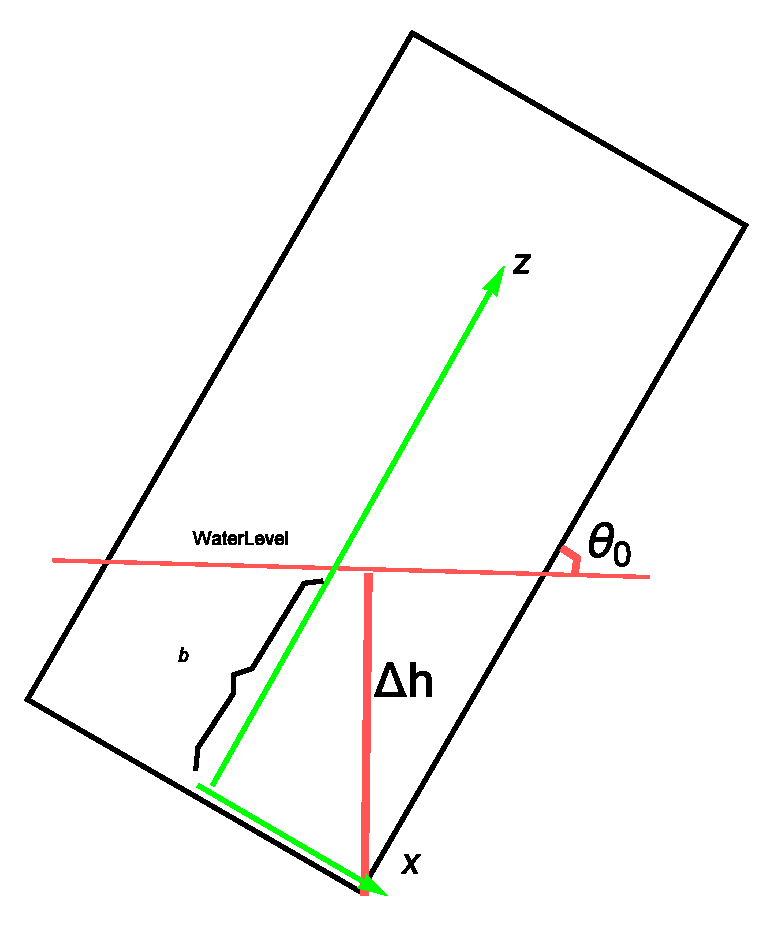
\includegraphics[width=200pt]{MyBuoy.eps}
\end{figure}

由平面几何的知识
可以求出水平面的直线方程为$z=\cot(\theta_0)x+b,b=\frac{\Delta h}{\sin(\theta_0)}-\frac{d_1 \cot(\theta_0)}{2}$,由割补法可得浮标圆柱的排水体积为$V_{buoy}=\pi (\frac{d_1}{2})^2 b$,在这种情况下我们还需要求出浮力的作用点即浮标的浮心,在$z-x$坐标
系中,由对称性可知浮心应位于$z$轴上,其坐标为
\begin{equation}
z_{buoyancy}=\frac{\iiint_{V_{buoy}} z\,dx\,dy\,dz}{V_{buoy}}
\end{equation}
通过累次积分和极坐标变换可求出$z_{buoyancy}=\frac{16 b^2+d_1^2 \cot^2(\theta_0)}{32b}$\\
下面考虑浮标水面上的部分在风向的法平面上的投影面积,
借助3维建模软件我们得到投影的形状为一个矩形和一个半椭圆的组合体
,椭圆长轴为$d_1$,短轴为$d_1 cos(theta_0)$
组合体的面积为:
\begin{equation}
S=d_1(h_1-b)\sin(\theta_0)+\frac{\pi d_1^2 \cos(\theta_0)}{8}
\end{equation}
于是在考虑浮标倾角的情况下,未知量只多出了$\theta_0$,而方程也相应的多出一个,即为浮标的力矩平衡方程(假设风力的等效作用点过质心,取浮标与第一节钢管的接触点为参考点).
\begin{equation}\label{BuoyTorqueEquilibrium}
F_{buoy}z_{buoyancy}\cos(\theta_0)+G_{buoy}\frac{h_1}{2}\cos(\theta_0)=F_{wind}\frac{h_1}{2}\sin(\theta_0)
\end{equation}
于是模型1中只需求解多了一个未知参量$\theta_0$和方程\ref{BuoyTorqueEquilibrium}的方程组即可得到模型3的结果。
\subsubsection{模型求解}
由以上的理论公式采用代入消元的方法将方程组化到未知量个数为2,编写函数 'ConsideringTiltingOfBuoy.m',用Matlab的fsolver分别对$v=12,24,36m/s$的风速求解,得到下
表:
\begin{table}[!ht]
\centering
\caption{倾斜模型计算结果与力学模型}
\begin{tabular}{c cc cc cc}
\hline \hline
\multicolumn{1}{c}{参数} & \multicolumn{2}{c}{$v_w=12m/s$} & \multicolumn{2}{c}{$v_w=24m/s$} & \multicolumn{2}{c}{$v_w=24m/s$}\\
\multicolumn{1}{c}{是否考虑浮标倾斜} & 否 & 是& 否& 是& 否& 是\\
\hline
$\theta_0$ & $90.00^{\circ}$ & $89.2823^{\circ}$ & $90.0^{\circ}$ & $87.1565^{\circ}$					& $90.000^{\circ}$ & $83.7336^{\circ}$\\
$\theta_1$ & $89.0226^{\circ}$ & $89.0152^{\circ}$ & $86.2640^{\circ}$ & $86.1582^{\circ}$					& $82.1546^{\circ}$ & $81.7225^{\circ}$\\
$\theta_2$ & $89.0168^{\circ}$ & $89.0094^{\circ}$ & $86.2428^{\circ}$ & $86.1364^{\circ}$               & $82.1124^{\circ}$ & $81.6783^{\circ}$\\
$\theta_3$ & $89.0110^{\circ}$ & $89.0035^{\circ}$ & $86.2213^{\circ}$ & $86.1143^{\circ}$             & $82.0698^{\circ}$ & $81.6337^{\circ}$\\
$\theta_4$ & $89.0051^{\circ}$ & $88.9976^{\circ}$ & $86.1995^{\circ}$ & $86.0919^{\circ}$           & $82.0267^{\circ}$ & $81.5886^{\circ}$\\
$\theta_5$ & $88.9917^{\circ}$ & $88.9841^{\circ}$ & $86.1502^{\circ}$ & $86.0413^{\circ}$               & $81.9292^{\circ}$ & $81.4864^{\circ}$\\
$a$        & $3.3198$          & $3.345$           & $13.1308$  		 &	$13.5186$					 & $29.0460$ 	  & $30.8374$  \\
$x_1$      & $7.3967$          & $7.4329$          & $16.7797$ 		    & $17.0550$    & $27.2596$         & $28.4135$   \\                               
$x_0$      & $0$               & $0$               & $0$ 					 & $0$   & $9.2348 $ 	  & $10.3619$  \\
$\theta_6$ & $0$               & $0$               & $0$                & $0$   & $17.9107$         & $19.6168$ \\
$\delta h$ & $0.7348$          & $0.7348$          & $0.7489$           & $0.7485$ & $0.7700 $         & $0.7679 $  \\
$R_{move}$ & $8.4832$          & $8.5199$          & $18.1097$          & $18.3931$  & $19.7156$         & $19.7741$\\

\hline \hline
\end{tabular}
\end{table}
由上表可看出,考虑倾角时结果与不考虑时相差不大,但随着风力的增大,二者的差别越来越明显
m
\subsection{模型5——离散情形:锚链视为由一节节小的链环组成}
\subsubsection{模型分析}
在以上模型的分析中,均将锚链视为连续介质,但实际计算组成锚链的链环个数时,问题(一)中只有210个链环,为更精确地描述整个系统,应为这210个链环分别设出倾斜角度,为讨论方便,假设共有$n$个链环,每节链环的长度设为$l_u$,链环倾角为$\alpha_i,i=1,..n$,沿用模型2的记号,仍假设锚点为坐标原点,第$j$个锚链的坐标为
\begin{equation}
\overrightarrow{r_j}=(l_u(\sum_{k=1}^{j-1} \cos(\alpha_k)+\frac{1}{2}\cos(\alpha_j)),
l_u(\sum_{k=1}^{j-1} \sin(\alpha_k) +\frac{1}{2}\sin(\alpha_j)))
\end{equation}
锚链的重力势能为$E_{Gcable}=\rho_{cable}g \sum_{j=1}^n \overrightarrow{r_j} \cdot \hat{y_j}$
将模型2中的$y(x_{end})$改为$\overrightarrow{r_n} \cdot \hat{y_n}$,系统其他节点的能量表达式不变,于是可得到
$$V=V(\alpha_1,..\alpha_n,\theta_0,..\theta_5,\Delta h),\text{constained by (\ref{WaterDepthConstraint}})$$
$\Delta h$可通过等式约束消元,于是问题转化为求一个只依赖$n+6$个角度参量的广义势函数的极小值。通过求此函数的驻点
可将问题进一步转化为求解高维非线性方程组。




\begin{thebibliography}{8}

\bibitem{catenery} Catenary, en.wikipedia.org/wiki/Catenary, September 10, 2016
\bibitem{DK86} D.E. Knuth, \emph{The {\TeX}book},  New Jersey, United States: Pearson Education (US), 1986
\bibitem{DK89} D.E. Knuth, \emph{Typesetting Concrete Mathematics}, Addison-Wesley Professional; 2 edition (March 10, 1994)
\bibitem{D01} 罗万成 \textsl{大学生数学建模案例精选}, 西南交通大学出版社,第1版, 2007

\end{thebibliography}




\newpage

\section{附录}
\begin{footnotesize}
\noindent \textbf{程序语言}:matlab;\textbf{文件}:launcher.m

\noindent \textbf{自定义函数}:func.m, func\_0.m, func3.m, func3\_0.m\\

\noindent \textbf{Launcher:  launcher.m}

\begin{lstlisting}[ language=matlab]
clear,clc;
warning off all;

global g;%gravity acceleration
global rho;%density of the sea
global v_w;%velocity of the wind
global h_w;%total depth of the sea
global rho_cable;%density of the cable
global h_1;%height of the buoy
global d_1;%diameter of the bottom surface of the buoy cylinder
global G_fb;%gravity of the buoy
global h_2;%length of the steel pipe
global d_2;%diameter of the bottom surpface of the steel pipe cylinder
global G_fbi;%gravity of the steel tube
global F_fbi;%buoyancy of the steel tube
global h_3;%height of the bucket
global d_3;%outer diameter of the bucket
global G_buc;%gravity of the bucket
global F_buc;%buoyancy of the bucket
global G_ball;%gavity of the ball
global L_cable;%the length of protracted cable


g = 9.8;
rho = 1025;
h_1 = 2;
d_1 = 2;
G_fb = 1000 * g;
h_2 = 1;
d_2 = 0.05;
G_fbi = 10 * g;
F_fbi = rho * g * h_2 * (d_2/2) ^ 2 * pi;
h_3 = 1;
d_3 = 0.3;
G_buc = 100 *g;
F_buc = rho * g * h_3 * (d_3/2) ^ 2 * pi;


%%
%question_1&2

v_w = 36;
h_w = 18;
rho_cable = 7;
L_cable = 22.05;
G_ball = 1200 *g;

%initialize results vars
global W_ball_all
global theta_5_all
global theta_6_all
W_ball_all = zeros(1,1);
theta_5_all = zeros(1,1);
theta_6_all = zeros(1,1);

for i = 1:1

    G_ball = (3200+50*(i-1))*g;
    W_ball_all(i) = G_ball/g;

    %  solve
    function_used = 1;%0-func_0;others-func
    h=optimset;
    h.MaxFunEvals=20000;
    h.MaxIter=10000;
    h.Display='on';
    if(function_used == 1)
        x=fsolve('func',[0.5,1.5,1.5,1.5,1.5,1.5],h);
    else
        x=fsolve('func_0',[0.5,1.5,1.5,1.5,1.5,1.5],h);
    end

    %solutions
    dh = x(1);
    theta_1 = x(2);
    theta_2 = x(3);
    theta_3 = x(4);
    theta_4 = x(5);
    theta_5 = x(6);

    %calculation
    V_s = dh * (d_1/2) ^ 2 * pi;%volume of the buoy under water level
    S_w = (h_1 - dh) * d_1;%projected surface area of the buoy along...
    ... the normal direction of the wind
    F_w = 0.625 * S_w * v_w ^ 2;%force exerced by the wind on the buoy
    F_fb = rho * g * V_s;%buoyancy of the buoy
    Y_10 = F_fb - G_fb;%vertical T_10
    Y_21 = Y_10 + F_fbi - G_fbi;%vertical T_21
    Y_32 = Y_21 + F_fbi - G_fbi;%vertical T_32
    Y_43 = Y_32 + F_fbi - G_fbi;%vertical T_43
    Y_54 = Y_43 + F_fbi - G_fbi;%vertical T_54
    Y = Y_54 + F_buc - G_ball - G_buc;%vertical T

    %catenary
    a = F_w/(rho_cable * g);
    x_1 = a * asinh(Y/F_w);

    %other results related to function types
    if(function_used == 1)
        h_4 = a * cosh(x_1/a)-sqrt(a ^ 2 + (L_cable - a * sinh(x_1/a))^2);
        x_0 = a * asinh(sinh(x_1/a)-L_cable/a);
        theta_6_angle = atan(sinh(x_0/a))/pi*180;
        theta_6_all(i) = theta_6_angle;
    else
        x_0 = 0;
        h_4 = a * (cosh(x_1/a)-1);
        L_cable_ = a* sinh(x_1/a);
    end

    %question_1&2, single Weight_ball
    theta_1_angle = theta_1 / pi * 180
    theta_2_angle = theta_2 / pi * 180
    theta_3_angle = theta_3 / pi * 180
    theta_4_angle = theta_4 / pi * 180
    theta_5_angle = theta_5 / pi * 180
    R_move = (x_1 - x_0) + h_3 * cos(theta_5) + h_2 * (cos(theta_1)+...
    ...cos(theta_2)+cos(theta_3)+cos(theta_4))+ d_1/2

    %question_2 only
%     theta_5_angle = theta_5 / pi * 180;
%     theta_5_all(i) = theta_5_angle;
%     yyy(i) = h_w-h_4-h_3*sin(theta_5)-h_2 * (sin(theta_1)+...
%...sin(theta_2)+sin(theta_3)+sin(theta_4))-dh;
end

%%
%question_3

global angle
global v_s

rho_cable_types = [28.12];
%rho_cable_types = 3.2;
L_cable_types = 16:0.5:30;
G_ball_types = 1000:200:4000;
h_w_types = 16:1:20;
v_w_types = 6:6:36;
v_s_types = 0:0.3:1.5;
angle_types = 0:30:150;
Results=zeros(length(rho_cable_types),length(L_cable_types),...
...length(G_ball_types));

for i = 1:length(rho_cable_types)
    for j = 1:length(L_cable_types)
        for k = 1:length(G_ball_types)
            disp([i, j, k]);

            rho_cable = rho_cable_types(i);
            L_cable = L_cable_types(j);
            G_ball = G_ball_types(k) * g;

            for l = 1:length(h_w_types)
                for m = 1:length(v_w_types)
                    for n = 1:length(v_s_types)
                        for o = 1:length(angle_types)

                            h_w = h_w_types(l);
                            v_w = v_w_types(m);
                            v_s = v_s_types(n);
                            angle = angle_types(o);

                            %solve
                            h=optimset;
                            h.MaxFunEvals=20000;
                            h.MaxIter=10000;
                            h.Display='off';
                            [x,y,if_solve] = fsolve('func3',[0.5...
                            ...,1.5,1.5,1.5,1.5,1.5],h);

                            %solutions
                            dh = x(1);
                            S_w = (h_1 - dh) * d_1;
                            S_s = dh * d_1;
                            F_w = 0.625 * S_w * v_w ^ 2;
                            F_s = 374 * S_s * v_s ^ 2;
                            F_ws = sqrt(F_w ^ 2 + F_s ^ 2 + 2 * F_w...
                            ... * F_s * cos(angle / 180 * pi));
                            a = F_ws/(rho_cable * g);
                            V_s = dh * (d_1/2) ^ 2 * pi;
                            F_fb = rho * g * V_s;
                            Y_10 = F_fb - G_fb;
                            Y_21 = Y_10 + F_fbi - G_fbi;
                            Y_32 = Y_21 + F_fbi - G_fbi;
                            Y_43 = Y_32 + F_fbi - G_fbi;
                            Y_54 = Y_43 + F_fbi - G_fbi;
                            Y = Y_54 + F_buc - G_ball - G_buc;
                            x_1 = a * asinh(Y/F_ws);
                            x_0 = a * asinh(sinh(x_1/a)-L_cable/a);

                            if((x_0 >= 0) && (if_solve == 1))
                                theta_1 = x(2);
                                theta_2 = x(3);
                                theta_3 = x(4);
                                theta_4 = x(5);
                                theta_5 = x(6);
                                theta_6_angle = atan(sinh(x_0/a))...
                                .../pi*180;

                                %calculation
                                R_move = (x_1 - x_0) + h_3 * ...
                                ...cos(theta_5) + h_2 * (cos...
                                ...(theta_1)+cos(theta_2)+cos...
                                ...(theta_3)+cos(theta_4))+ d_1/2;
                                temp = (dh/h_1)^ 2 + (R_move/30)...
                                ...^ 2 + ((90-theta_5/pi*180)/5)...
                                ...^ 2 + max(theta_6_angle-16,0);
                                Results(i,j,k) = Results(i,j,k)+...
                                ... temp/(length(h_w_types)*...
                                ...length(v_w_types)*length...
                                ...(v_s_types)*length(angle_types));
                            else
                                %solve
                                h=optimset;
                                h.MaxFunEvals=20000;
                                h.MaxIter=10000;
                                h.Display='off';
                                [x,y,if_solve]=fsolve('func3_0',...
                                ...[0.5,1.5,1.5,1.5,1.5,1.5],h);
                                dh = x(1);
                                S_w = (h_1 - dh) * d_1;
                                S_s = dh * d_1;
                                F_w = 0.625 * S_w * v_w ^ 2;
                                F_s = 374 * S_s * v_s ^ 2;
                                F_ws = sqrt(F_w ^ 2 + F_s ^ 2 + 2...
                                ... * F_w * F_s * cos(angle / 180 * pi));
                                a = F_ws/(rho_cable * g);
                                V_s = dh * (d_1/2) ^ 2 * pi;
                                F_fb = rho * g * V_s;
                                Y_10 = F_fb - G_fb;
                                Y_21 = Y_10 + F_fbi - G_fbi;
                                Y_32 = Y_21 + F_fbi - G_fbi;
                                Y_43 = Y_32 + F_fbi - G_fbi;
                                Y_54 = Y_43 + F_fbi - G_fbi;
                                Y = Y_54 + F_buc - G_ball - G_buc;
                                x_1 = a * asinh(Y/F_ws);
                                x_0 = 0;
                                L_cable_ = a* sinh(x_1/a);

                                if(((dh > h_1) || (L_cable_ > L_cable))...
                                ...|| (if_solve ~= 1))
                                    disp('wrong');
                                    disp([dh,L_cable_,if_solve]);
                                    disp([rho_cable,L_cable,G_ball,h_w,...
                                    ...v_w,v_s,angle]);
                                    Results(i,j,k) = Results(i,j,k) + 4;
                                else
                                    %disp('func_0');
                                    theta_1 = x(2);
                                    theta_2 = x(3);
                                    theta_3 = x(4);
                                    theta_4 = x(5);
                                    theta_5 = x(6);
                                    theta_6_angle = atan(sinh(x_0/a))/...
                                    ...pi*180;

                                    %calculation
                                    R_move = (x_1 - x_0) + h_3 * cos...
                                    ...(theta_5) + h_2 * (cos(theta_1)...
                                    ...+cos(theta_2)+cos(theta_3)+cos...
                                    ...(theta_4))+ d_1/2;
                                    temp = (dh/h_1)^ 2 + (R_move/30)^2+...
                                    ...((90-theta_5/pi*180)/5)^ 2 + max...
                                    ...(theta_6_angle-16,0);
                                    Results(i,j,k) = Results(i,j,k) + ...
                                    ...temp/(length(h_w_types)*length...
                                    ...(v_w_types)*length(v_s_types)...
                                    ...*length(angle_types));
                                end

                            end
                        end
                    end
                end
            end

        end
    end
end
%%
%find the min result
disp(final_esults);
disp(min(final_results(:)));
Lin=find(final_results<=min(final_results(:)));
[i,j,k]=ind2sub(size(final_results),Lin);
disp([i,j,k]);

\end{lstlisting}

\textbf{function:  func.m}

\begin{lstlisting}[ language=matlab]
function yyy = func(xxx)
global g;
global rho;
global v_w;
global h_w;
global rho_cable;
global h_1;
global d_1;
global G_fb;
global h_2;
global G_fbi;
global F_fbi;
global h_3;
global G_buc;
global F_buc;
global G_ball;
global L_cable;

dh = xxx(1);%assum
V_s = dh * (d_1/2) ^ 2 * pi;
S_w = (h_1 - dh) * d_1;
F_w = 0.625 * S_w * v_w ^ 2;
F_fb = rho * g * V_s;

Y_10 = F_fb - G_fb;
Y_21 = Y_10 + F_fbi - G_fbi;
Y_32 = Y_21 + F_fbi - G_fbi;
Y_43 = Y_32 + F_fbi - G_fbi;
Y_54 = Y_43 + F_fbi - G_fbi;
Y = Y_54 + F_buc - G_ball - G_buc;

a = F_w/(rho_cable * g);
x_1 = a * asinh(Y/F_w);
h_4 = a * cosh(x_1/a)-sqrt(a ^ 2 + (L_cable - a * sinh(x_1/a))^2);
%x_0 = a * asinh(sinh(x_1/a)-L_cable/a);

theta_1 = xxx(2);
theta_2 = xxx(3);
theta_3 = xxx(4);
theta_4 = xxx(5);
theta_5 = xxx(6);
yyy(1) = h_w-h_4-h_3*sin(theta_5)-h_2 * (sin(theta_1)+sin(theta_2)...
...+sin(theta_3)+sin(theta_4))-dh;
yyy(2) = (G_fbi - F_fbi)*cos(theta_1)/2 + F_w*sin(theta_1) - Y_10...
... * cos(theta_1);
yyy(3) = (G_fbi - F_fbi)*cos(theta_2)/2 + F_w*sin(theta_2) - Y_21...
... * cos(theta_2);
yyy(4) = (G_fbi - F_fbi)*cos(theta_3)/2 + F_w*sin(theta_3) - Y_32...
... * cos(theta_3);
yyy(5) = (G_fbi - F_fbi)*cos(theta_4)/2 + F_w*sin(theta_4) - Y_43...
... * cos(theta_4);
yyy(6) = (G_buc - F_buc)*cos(theta_5)/2 + F_w*sin(theta_5) - Y_54...
... * cos(theta_5);
yyy(7) = Y-abs(Y);% we request that T_v larger than
end
\end{lstlisting}

\newpage
\textbf{function:  func\_0.m}

\begin{lstlisting}[ language=matlab]

function yyy = func_0(xxx)
global g;
global rho;
global v_w;
global h_w;
global rho_cable;
global h_1;
global d_1;
global G_fb;
global h_2;
global G_fbi;
global F_fbi;
global h_3;
global G_buc;
global F_buc;
global G_ball;

dh = xxx(1);%assum
V_s = dh * (d_1/2) ^ 2 * pi;
S_w = (h_1 - dh) * d_1;

F_w = 0.625 * S_w * v_w ^ 2;
F_fb = rho * g * V_s;

Y_10 = F_fb - G_fb;
Y_21 = Y_10 + F_fbi - G_fbi;
Y_32 = Y_21 + F_fbi - G_fbi;
Y_43 = Y_32 + F_fbi - G_fbi;
Y_54 = Y_43 + F_fbi - G_fbi;
Y = Y_54 + F_buc - G_ball - G_buc;

a = F_w/(rho_cable * g);
x_1 = a * asinh(Y/F_w);
h_4 = a * (cosh(x_1/a)-1);

theta_1 = xxx(2);
theta_2 = xxx(3);
theta_3 = xxx(4);
theta_4 = xxx(5);
theta_5 = xxx(6);
yyy(1) = h_w-h_4-h_3*sin(theta_5)-h_2 * (sin(theta_1)+sin(theta_2)...
...+sin(theta_3)+sin(theta_4))-dh;
yyy(2) = (G_fbi - F_fbi)*cos(theta_1)/2 + F_w*sin(theta_1) - Y_10...
... * cos(theta_1);
yyy(3) = (G_fbi - F_fbi)*cos(theta_2)/2 + F_w*sin(theta_2) - Y_21...
... * cos(theta_2);
yyy(4) = (G_fbi - F_fbi)*cos(theta_3)/2 + F_w*sin(theta_3) - Y_32...
... * cos(theta_3);
yyy(5) = (G_fbi - F_fbi)*cos(theta_4)/2 + F_w*sin(theta_4) - Y_43...
... * cos(theta_4);
yyy(6) = (G_buc - F_buc)*cos(theta_5)/2 + F_w*sin(theta_5) - Y_54...
... * cos(theta_5);
yyy(7) = Y-abs(Y);
end
\end{lstlisting}


\newpage
\textbf{function:  func3.m}

\begin{lstlisting}[ language=matlab]
function yyy = func3(xxx)
global g;
global rho;
global v_w;
global h_w;
global rho_cable;
global h_1;
global d_1;
global G_fb;
global h_2;
global G_fbi;
global F_fbi;
global h_3;
global G_buc;
global F_buc;
global G_ball;
global L_cable;
global angle;
global v_s;

dh = xxx(1);%assum
V_s = dh * (d_1/2) ^ 2 * pi;
S_w = (h_1 - dh) * d_1;
S_s = dh * d_1;
F_w = 0.625 * S_w * v_w ^ 2;
F_s = 374 * S_s * v_s ^ 2;

F_fb = rho * g * V_s;

Y_10 = F_fb - G_fb;
Y_21 = Y_10 + F_fbi - G_fbi;
Y_32 = Y_21 + F_fbi - G_fbi;
Y_43 = Y_32 + F_fbi - G_fbi;
Y_54 = Y_43 + F_fbi - G_fbi;
Y = Y_54 + F_buc - G_ball - G_buc;

F_ws = sqrt(F_w ^ 2 + F_s ^ 2 + 2 * F_w * F_s * cos(angle / 180 * pi));
a = F_ws/(rho_cable * g);
x_1 = a * asinh(Y/F_ws);
h_4 = a * cosh(x_1/a)-sqrt(a ^ 2 + (L_cable - a * sinh(x_1/a))^2);

theta_1 = xxx(2);
theta_2 = xxx(3);
theta_3 = xxx(4);
theta_4 = xxx(5);
theta_5 = xxx(6);
yyy(1) = h_w-h_4-h_3*sin(theta_5)-h_2 * (sin(theta_1)+sin(theta_2)...
...+sin(theta_3)+sin(theta_4))-dh;
yyy(2) = (G_fbi - F_fbi)*cos(theta_1)/2 + F_w*sin(theta_1) - Y_10...
... * cos(theta_1);
yyy(3) = (G_fbi - F_fbi)*cos(theta_2)/2 + F_w*sin(theta_2) - Y_21...
... * cos(theta_2);
yyy(4) = (G_fbi - F_fbi)*cos(theta_3)/2 + F_w*sin(theta_3) - Y_32...
... * cos(theta_3);
yyy(5) = (G_fbi - F_fbi)*cos(theta_4)/2 + F_w*sin(theta_4) - Y_43...
... * cos(theta_4);
yyy(6) = (G_buc - F_buc)*cos(theta_5)/2 + F_w*sin(theta_5) - Y_54...
... * cos(theta_5);
yyy(7) = Y-abs(Y);
end
\end{lstlisting}

\textbf{function:  func3\_0.m}

\begin{lstlisting}[ language=matlab]
function yyy = func3_0(xxx)
global g;
global rho;
global v_w;
global h_w;
global rho_cable;
global h_1;
global d_1;
global G_fb;
global h_2;
global G_fbi;
global F_fbi;
global h_3;
global G_buc;
global F_buc;
global G_ball;
global angle;
global v_s;


dh = xxx(1);%assum
V_s = dh * (d_1/2) ^ 2 * pi;
S_w = (h_1 - dh) * d_1;
S_s = dh * d_1;
F_s = 374 * S_s * v_s ^ 2;
F_w = 0.625 * S_w * v_w ^ 2;
F_fb = rho * g * V_s;

Y_10 = F_fb - G_fb;
Y_21 = Y_10 + F_fbi - G_fbi;
Y_32 = Y_21 + F_fbi - G_fbi;
Y_43 = Y_32 + F_fbi - G_fbi;
Y_54 = Y_43 + F_fbi - G_fbi;
Y = Y_54 + F_buc - G_ball - G_buc;

F_ws = sqrt(F_w ^ 2 + F_s ^ 2 + 2 * F_w * F_s * cos(angle / 180 * pi));
a = F_ws/(rho_cable * g);
x_1 = a * asinh(Y/F_ws);
h_4 = a * (cosh(x_1/a)-1);

theta_1 = xxx(2);
theta_2 = xxx(3);
theta_3 = xxx(4);
theta_4 = xxx(5);
theta_5 = xxx(6);
yyy(1) = h_w-h_4-h_3*sin(theta_5)-h_2 * (sin(theta_1)+sin(theta_2)...
...+sin(theta_3)+sin(theta_4))-dh;
yyy(2) = (G_fbi - F_fbi)*cos(theta_1)/2 + F_w*sin(theta_1) - Y_10...
... * cos(theta_1);
yyy(3) = (G_fbi - F_fbi)*cos(theta_2)/2 + F_w*sin(theta_2) - Y_21...
... * cos(theta_2);
yyy(4) = (G_fbi - F_fbi)*cos(theta_3)/2 + F_w*sin(theta_3) - Y_32...
... * cos(theta_3);
yyy(5) = (G_fbi - F_fbi)*cos(theta_4)/2 + F_w*sin(theta_4) - Y_43...
... * cos(theta_4);
yyy(6) = (G_buc - F_buc)*cos(theta_5)/2 + F_w*sin(theta_5) - Y_54...
... * cos(theta_5);
yyy(7) = Y-abs(Y);
end
\end{lstlisting}
\textbf{function:  ConsideringTiltingOfBuoy.m}

\begin{lstlisting}[language=matlab]
function output = ConsideringTiltingOfBuoy(delta_h,theta_0,v)
global g;%gravity acceleration
global rho;%density of the sea
global h_w;%total depth of the sea
global rho_cable;%density of the cable
global h_1;%height of the buoy
global d_1;%diameter of the bottom surface of the buoy cylinder
global G_tube;%gravity of the steel tube
global F_tube;%buoyancy of the steel tube
global G_buc;%gravity of the bucket
global F_buc;%buoyancy of the bucket
global G_buoy;%gravity of the buoy
global L_cable;
global G_ball;
global h_3;%height of the bucket
global h_2;%length of the steel pipe

b=delta_h/sin(theta_0);
Surface=d_1*sin(theta_0)*(h_1-b)+pi*d_1^2*cos(theta_0)/8;
Fw = 0.625*Surface*v^2;
z_buoyancy=b/2+d_1^2*cot(theta_0)^2/(32*b);
a = Fw/(rho_cable*g);
Fbuoy =b*g*rho*pi*(d_1/2)^2;
t1 = (2*(Fbuoy-G_buoy) + (F_tube -G_tube))/sqrt((2*(Fbuoy -G_buoy)
 + (F_tube -G_tube))^2 + 4*Fw^2);
t2 = (2*Fbuoy + 3*F_tube - 2*G_buoy - 3*G_tube)
/sqrt((2*Fbuoy + 3*F_tube - 2*G_buoy - 3*G_tube)^2 + 4*Fw^2);
t3 = (2*Fbuoy + 5*F_tube - 2*G_buoy - 5*G_tube) 
/sqrt((2*Fbuoy + 5*F_tube - 2*G_buoy - 5*G_tube) ^2 + 4*Fw^2);
t4 = (2*Fbuoy + 7*F_tube - 2*G_buoy - 7*G_tube)
/sqrt((2*Fbuoy + 7*F_tube - 2*G_buoy - 7*G_tube)^2 + 4*Fw^2);
t5 = (F_buc + 2*Fbuoy + 8*F_tube - G_buc - 2*G_buoy - 8*G_tube)
/sqrt((F_buc + 2*Fbuoy + 8*F_tube - G_buc - 2*G_buoy - 8*G_tube)^2 + 4*Fw^2);
h4 = h_w - (h_3*t5 + h_2*(t1 + t2 + t3 + t4) + delta_h);
x1 = a*asinh(sqrt((L_cable^2 - h4^2)/(4*a^2))) 
+ 0.5*a*acosh((L_cable^2 + h4^2)/(L_cable^2 - h4^2));
x0 = -a*asinh(sqrt((L_cable^2 - h4^2)/(4*a^2))) 
+0.5*a*acosh((L_cable^2 + h4^2)/(L_cable^2 - h4^2));
if(x0 < 0)
    x1 = a*(acosh(h4/a + 1));
    x0=0;
end
 output(1)=(F_buc + Fbuoy + 4*F_tube - G_ball
 - G_buc -G_buoy - 4*G_tube)/Fw - sinh(x1/a);
 output(2)=Fbuoy*z_buoyancy*cos(theta_0)
 +G_buoy*h_1*0.5*cos(theta_0)-Fw*h_1*0.5*sin(theta_0);
end
\end{lstlisting}

\textbf{Mathematica.nb: NonLinearSolver}

\begin{lstlisting}[language=Mathematica]
SolverFunction[\[CapitalDelta]h_,v_]:=Module[{Fw,a,Fbuoy,t1,t2,t3,t4,t5,h4,x1,x0},
Fw=0.625*(h1-\[CapitalDelta]h)*d1*v^2;
a=Fw/(\[Rho]cable*g);
Fbuoy=\[CapitalDelta]h*g*\[Rho]w*\[Pi]*(d1/2)^2;
t1=(2(Fbuoy-Gbuoy)+(Fp-Gp))/Sqrt[(2(Fbuoy-Gbuoy)+(Fp-Gp))^2+4*Fw^2];
t2=(2 Fbuoy+3 Fp-2 Gbuoy-3 Gp)/Sqrt[(2 Fbuoy+3 Fp-2 Gbuoy-3 Gp)^2+4*Fw^2];
t3=(2 Fbuoy+5 Fp-2 Gbuoy-5 Gp) /Sqrt[(2 Fbuoy+5 Fp-2 Gbuoy-5 Gp) ^2+4*Fw^2];
t4=(2 Fbuoy+7 Fp-2 Gbuoy-7 Gp)/Sqrt[(2 Fbuoy+7 Fp-2 Gbuoy-7 Gp)^2+4*Fw^2];
t5=(Fbuc+2 Fbuoy+8 Fp-Gbuc-2 Gbuoy-8 Gp)/
Sqrt[(Fbuc+2 Fbuoy+8 Fp-Gbuc-2 Gbuoy-8 Gp)^2+4*Fw^2];
h4=hw-(h3*t5+h2*(t1+t2+t3+t4)+\[CapitalDelta]h);
x1=a*ArcSinh[Sqrt[(Lcable^2-h4^2)/(4*a^2)]]+
a/2 ArcCosh[(Lcable^2+h4^2)/(Lcable^2-h4^2)];
x0=-a*ArcSinh[Sqrt[(Lcable^2-h4^2)/(4*a^2)]]+
a/2 ArcCosh[(Lcable^2+h4^2)/(Lcable^2-h4^2)];
If[x0<0,x1=a*(ArcCosh[h4/a+1])];
(Fbuc+Fbuoy+4 Fp-Gball-Gbuc-Gbuoy-4 Gp)/Fw-Sinh[x1/a]]

(*Use dichotomy Method to find the solution of Solver*)
NonLinearSolver[w1s_,w2s_,iterativeTimes_,vs_]:=
Module[{\[CapitalDelta]h,w1,w2,v,iterativeTime},
w1=w1s;w2=w2s;v=vs;iterativeTime=iterativeTimes;
\[CapitalDelta]h=(w1+w2)/2;If[SolverFunction[w1,v]<0
&&SolverFunction[w2,v]>0,
For[j=1,j<iterativeTime,j++,
If[SolverFunction[\[CapitalDelta]h,v]<0,w1=\[CapitalDelta]h,
w2=\[CapitalDelta]h];\[CapitalDelta]h=(w1+w2)/2],If[SolverFunction[w1,v]>0&&
SolverFunction[w2,v]<0,For[j=1,j<iterativeTime,j++,
If[SolverFunction[\[CapitalDelta]h,v]<0,w2=\[CapitalDelta]h,w1=\[CapitalDelta]h];
\[CapitalDelta]h=(w1+w2)/2],
Throw["The function at the interval boundary points has the same sign!"]]];
Catch[\[CapitalDelta]h]]



(*By requiring all force component and angle componnt large than zero,
we can obtain the lower limit of \[CapitalDelta]h*)
Off[Reduce::ratnz]
Fbuoy=\[CapitalDelta]h*g*\[Rho]w*\[Pi]*(d1/2)^2;
Reduce[{2(Fbuoy-Gbuoy)+(Fp-Gp)>0,
(2 Fbuoy+3 Fp-2 Gbuoy-3 Gp)>0,
(2 Fbuoy+5 Fp-2 Gbuoy-5 Gp) >0,
(2 Fbuoy+7 Fp-2 Gbuoy-7 Gp)>0,
(Fbuc+2 Fbuoy+8 Fp-Gbuc-2 Gbuoy-8 Gp)>0,Fbuoy-Gbuoy>0,
Fbuoy+Fp-Gbuoy-Gp>0,Fbuoy+2 Fp-Gbuoy-2 Gp>0,Fbuoy+3 Fp-Gbuoy-3 Gp>0,
Fbuoy+4 Fp-Gbuoy-4 Gp>0,Fbuc+Fbuoy+4 Fp-Gball-Gbuc-Gbuoy-4 Gp>0}
,\[CapitalDelta]h]
\[CapitalDelta]h>0.701678
\end{lstlisting}

\textbf{Modeling.nb contains basic modeing equation}
\begin{lstlisting}[language=Mathematica]
(*Initial Parameter*)
g=9.8;
\[Rho]cable=7;
Lcable=22.05;
Gball=1200*g;
\[Rho]w=1025;
hw=18;
h2=1;
d2=0.05;
Gp=10*g;
d1=2;
h1=2;
Gbuoy=1000*g;
h3=1;
d3=0.3;
Gbuc=100*g;
Fp=\[Pi]*\[Rho]w*g*h2*(d2/2)^2;
Fbuc=\[Pi]*\[Rho]w*g*h3*(d3/2)^2;

(*Because of the complexity of the equation system, 
the Mathematica Kernel can not solve it directly*)
NSolve[{S==(h1-\[CapitalDelta]h)*d1,Fw==0.625*S*v^2,
hw==h4+h3*Sin[\[Theta]5]+h2*(Sin[\[Theta]1]+Sin[\[Theta]2]+
Sin[\[Theta]3]+Sin[\[Theta]4])+\[CapitalDelta]h,
h4==a*(Cosh[x1/a]-Cosh[x0/a]),Rv/Fw==Sinh[x1/a],
a==Fw/(\[Rho]cable*g),Lcable==a*(Sinh[x1/a]-Sinh[x0/a]),
Fbuoy==Gbuoy+Rv1,Fbuoy==\[CapitalDelta]h*g*\[Rho]w*\[Pi]*(d1/2)^2,
Rv1+Fp==Rv2+Gp,
(Gp-Fp)*Cos[\[Theta]1]/2+Fw*Sin[\[Theta]1]==Rv1*Cos[\[Theta]1],
Rv2+Fp==Rv3+Gp,(Gp-Fp)*Cos[\[Theta]2]/2+Fw*Sin[\[Theta]2]==Rv2*Cos[\[Theta]2],
Rv3+Fp==Rv4+Gp,(Gp-Fp)*Cos[\[Theta]3]/2+Fw*Sin[\[Theta]3]==Rv3*Cos[\[Theta]3],
Rv4+Fp==Gp+Rv5,(Gp-Fp)*Cos[\[Theta]4]/2+Fw*Sin[\[Theta]4]==Rv4*Cos[\[Theta]4],
Rv5+Fbuc==Rv+Gball+Gbuc,
(Gbuc-Fbuc)*Cos[\[Theta]5]/2+Fw*Sin[\[Theta]5]==Rv5*Cos[\[Theta]5]},
{\[CapitalDelta]h,S,Fw,h4,\[Theta]1,\[Theta]2,\[Theta]3,\[Theta]4,
\[Theta]5,x1,x0,a,Tv,Fbuoy,T10v,T21v,T32v,T43v,T54v}]

(*Below we represent the reaction force as the buoyancy and gravity force*)
Solve[{Fbuoy==Gbuoy+Rv1,
Rv1+Fp==Rv2+Gp,
Rv2+Fp==Rv3+Gp,
Rv3+Fp==Rv4+Gp,
Rv4+Fp==Gp+Rv5,
Rv5+Fbuc==Rv+Gball+Gbuc},{Rv1,Rv2,Rv3,Rv4,Rv5,Rv}]

{{Rv1->Fbuoy-Gbuoy,Rv2->Fbuoy+Fp-Gbuoy-Gp,Rv3->Fbuoy+2 
Fp-Gbuoy-2 Gp,
Rv4->Fbuoy+3 Fp-Gbuoy-3 Gp,Rv5->Fbuoy+4 Fp-Gbuoy-4 Gp,
Rv->Fbuc+Fbuoy+4 Fp-Gball-Gbuc-Gbuoy-4 Gp}}
(*Then we insert the expression of reaction force into equations
 about \[Theta]1 to \[Theta]5*)
{1/2 (-Fp+Gp) Cos[\[Theta]1]+Fw Sin[\[Theta]1]-Rv1 Cos[\[Theta]1],
1/2 (-Fp+Gp) Cos[\[Theta]2]+
Fw Sin[\[Theta]2]-Rv2 Cos[\[Theta]2],1/2 (-Fp+Gp) Cos[\[Theta]3]+
Fw Sin[\[Theta]3]-Rv3 Cos[\[Theta]3],
1/2 (-Fp+Gp) Cos[\[Theta]4]+Fw Sin[\[Theta]4]-Rv4 Cos[\[Theta]4],
1/2 (-Fbuc+Gbuc) Cos[\[Theta]5]+Fw Sin[\[Theta]5]-Rv5 Cos[\[Theta]5]}/.\%//Simplify
{{-(1/2) (2 Fbuoy+Fp-2 Gbuoy-Gp) Cos[\[Theta]1]+Fw Sin[\[Theta]1],(-Fbuoy-(3 Fp)/2
+Gbuoy+(3 Gp)/2) Cos[\[Theta]2]+Fw Sin[\[Theta]2],(
-Fbuoy-(5 Fp)/2+Gbuoy+(5 Gp)/2) Cos[\[Theta]3]+Fw Sin[\[Theta]3],(-Fbuoy-(7 Fp)/2
+Gbuoy+(7 Gp)/2) Cos[\[Theta]4]+
Fw Sin[\[Theta]4],-(1/2) (Fbuc+2 Fbuoy+8 Fp-Gbuc-2 Gbuoy-8 Gp)
Cos[\[Theta]5]+Fw Sin[\[Theta]5]}}
(*We can reduce the function to one dimension about \[CapitalDelta]h*)
Tan[\[Theta]1]=(2(Fbuoy-Gbuoy)+(Fp-Gp))/(2*Fw);
Tan[\[Theta]2]=(2 Fbuoy+3 Fp-2 Gbuoy-3 Gp) /(2*Fw);
Tan[\[Theta]3]=(2 Fbuoy+5 Fp-2 Gbuoy-5 Gp) /(2*Fw);
Tan[\[Theta]4]=(2 Fbuoy+7 Fp-2 Gbuoy-7 Gp) /(2*Fw);
Tan[\[Theta]5]=(Fbuc+2 Fbuoy+8 Fp-Gbuc-2 Gbuoy-8 Gp) /(2*Fw);
ArcSinh[Sqrt[(Lcable^2-h4^2)/(4*a^2)]]==(x1-x0)/(2 a);
ArcCosh[(Lcable^2+h4^2)/(Lcable^2-h4^2)]== (x0+x1)/a ;
(*From the above two equation, we can solve out x1*)
x1=a*ArcSinh[Sqrt[(Lcable^2-h4^2)/(4*a^2)]]-a/2 
ArcCosh[(Lcable^2+h4^2)/(Lcable^2-h4^2)];
x0=-a*ArcSinh[Sqrt[(Lcable^2-h4^2)/(4*a^2)]]+a/2 
ArcCosh[(Lcable^2+h4^2)/(Lcable^2-h4^2)];
(*where*)
a=(0.625*(h1-\[CapitalDelta]h)*d1*v^2)/(\[Rho]cable*g);
h4=hw-(h3*Sin[\[Theta]5]+h2*(Sin[\[Theta]1]+Sin[\[Theta]2]+
Sin[\[Theta]3]+Sin[\[Theta]4])+\[CapitalDelta]h);
(*Then we can reduce the equation system to one dimension,
see NonLinearSolver.nb for detail*)
\end{lstlisting}
\textbf{Modeling.nb contains basic modeing equation}
\begin{lstlisting}[language=Mathematica]
E1=\[Rho]cable*g*(Integrate[(\[Lambda]2+y[x])*Sqrt[1+y'[x]^2],
{x,0,xe}]-\[Lambda]2*Lcable)+y[xe]*Gball+(y[xe]+h3/2*Sin[\[Theta]5])*
(Gbuc-Fbuc)+(Gp-Fp)*((4*y[xe])+4*h3*Sin[\[Theta]5]+h2*((7 Sin[\[Theta]4])/2
+(5 Sin[\[Theta]3])/2+(3 Sin[\[Theta]2])/2+Sin[\[Theta]1]/2))
+(hw-\[CapitalDelta]h+h1/2)
*(Gbuoy-\[Pi]*(d1/2)^2*\[CapitalDelta]h*\[Rho]w*g)-(xe+h3*Cos[\[Theta]5]+
h2*(Cos[\[Theta]1]+Cos[\[Theta]2]+Cos[\[Theta]3]+Cos[\[Theta]4]))*K1
*d1*(h1-\[CapitalDelta]h)+\[Lambda]1*(hw-\[CapitalDelta]h-y[xe]-h2
*(Sin[\[Theta]1]+Sin[\[Theta]2]+Sin[\[Theta]3]+Sin[\[Theta]4])
-h3*Sin[\[Theta]5]);
(*Minimize this functional with y unknown, xe,\[Theta]1 to \[Theta]5,
\[CapitalDelta]h as general coordinates,*)
(*For the special case above, we can solve out the general
 form of the cable as follows:*)
y=a(Cosh[(x+x0)/a]-Cosh[x0/a]);xe=x1-x0;

\end{lstlisting}
val(:,:,1) =

   26.5690   17.0986   11.0548    7.1182    4.6698    3.2583    2.5681    2.2945
   19.6102   10.1623    5.2464    2.9143    1.9968    1.7371    1.7269    1.7472
   13.0903    5.1030    2.2187    1.4610    1.3738    1.3787    1.3818    1.3826
    8.1414    2.3917    1.2083    1.1241    1.1258    1.1262    1.1263    1.1263
    4.7978    1.2072    0.9337    0.9318    0.9319    0.9319    0.9319    0.9319


val(:,:,2) =

   25.8136   16.4310   10.4396    6.5211    4.1003    2.7350    2.0722    1.8340
   18.8307    9.5239    4.6934    2.4351    1.5791    1.3650    1.3590    1.3762
   12.3635    4.5696    1.8155    1.1473    1.0784    1.0822    1.0847    1.0854
    7.4950    2.0221    0.9641    0.8932    0.8948    0.8952    0.8952    0.8952
    4.2972    0.9752    0.7588    0.7575    0.7576    0.7576    0.7576    0.7576


val(:,:,3) =

   25.1740   15.9011    9.9783    6.0988    3.7179    2.3967    1.7627    1.5537
   18.1647    9.0231    4.2955    2.1178    1.3202    1.1401    1.1360    1.1517
   11.7421    4.1715    1.5542    0.9566    0.8973    0.9004    0.9026    0.9033
    6.9861    1.7550    0.8133    0.7505    0.7521    0.7525    0.7525    0.7525
    3.9128    0.8341    0.6502    0.6497    0.6498    0.6498    0.6498    0.6498


val(:,:,4) =

   24.5933   15.4459    9.5994    5.7818    3.4471    2.1646    1.5684    1.3769
   17.5703    8.6021    3.9904    1.8960    1.1520    1.0002    0.9979    1.0123
   11.1903    3.8690    1.3779    0.8379    0.7850    0.7878    0.7899    0.7905
    6.5790    1.5739    0.7189    0.6626    0.6643    0.6647    0.6647    0.6647
    3.6265    0.7500    0.5843    0.5844    0.5845    0.5845    0.5845    0.5845


val(:,:,5) =

   24.0576   15.0434    9.2750    5.5300    3.2400    2.0037    1.4399    1.2678
   17.0316    8.2545    3.7542    1.7434    1.0415    0.9135    0.9124    0.9262
   10.6872    3.6335    1.2679    0.7642    0.7166    0.7194    0.7214    0.7219
    6.2090    1.4600    0.6616    0.6108    0.6124    0.6127    0.6127    0.6127
    3.3787    0.7003    0.5473    0.5478    0.5479    0.5479    0.5479    0.5479


val(:,:,6) =

   23.5400   14.6723    8.9847    5.3114    3.0869    1.8907    1.3608    1.2026
   16.5180    7.9382    3.5795    1.6435    0.9811    0.8616    0.8614    0.8748
   10.2319    3.4437    1.1957    0.7213    0.6775    0.6807    0.6826    0.6831
    5.8711    1.3788    0.6305    0.5836    0.5852    0.5855    0.5855    0.5855
    3.1622    0.6769    0.5305    0.5313    0.5314    0.5314    0.5314    0.5314


val(:,:,7) =

   23.0379   14.3108    8.7168    5.1245    2.9698    1.8157    1.3138    1.1658
   16.0174    7.6547    3.4385    1.5768    0.9544    0.8336    0.8338    0.8473
    9.8131    3.3030    1.1518    0.7009    0.6590    0.6627    0.6647    0.6652
    5.5636    1.3290    0.6175    0.5739    0.5755    0.5758    0.5758    0.5758
    2.9843    0.6721    0.5286    0.5295    0.5296    0.5296    0.5296    0.5296


val(:,:,8) =

   22.5328   13.9640    8.4679    4.9668    2.8807    1.7727    1.2894    1.1488
   15.5337    7.4064    3.3313    1.5443    0.9483    0.8222    0.8230    0.8371
    9.4300    3.1879    1.1476    0.6961    0.6555    0.6599    0.6619    0.6624
    5.3286    1.3145    0.6186    0.5772    0.5789    0.5791    0.5791    0.5791
    2.8645    0.6849    0.5378    0.5388    0.5388    0.5388    0.5388    0.5388


val(:,:,9) =

   22.0347   13.6186    8.2364    4.8293    2.8104    1.7504    1.2884    1.1478
   15.0652    7.1727    3.2461    1.5343    0.9555    0.8231    0.8248    0.8397
    9.0900    3.0960    1.1615    0.7029    0.6632    0.6685    0.6706    0.6710
    5.1400    1.3273    0.6301    0.5904    0.5922    0.5925    0.5925    0.5925
    2.7825    0.7081    0.5556    0.5566    0.5567    0.5567    0.5567    0.5567


val(:,:,10) =

   21.5342   13.2649    8.0105    4.7061    2.7616    1.7477    1.3000    1.1569
   14.6020    6.9586    3.1839    1.5500    0.9750    0.8331    0.8363    0.8521
    8.7917    3.0529    1.1879    0.7197    0.6798    0.6860    0.6882    0.6887
    4.9659    1.3565    0.6493    0.6115    0.6134    0.6137    0.6137    0.6137
    2.7189    0.7388    0.5803    0.5814    0.5814    0.5814    0.5814    0.5814


val(:,:,11) =

   21.0234   16.9153    7.7904    4.6076    2.7290    1.7561    1.3211    1.1741
   14.1337    6.7721    3.1476    1.5871    1.0023    0.8511    0.8554    0.8724
    8.4915    3.0381    1.2271    0.7448    0.7036    0.7105    0.7130    0.7135
    4.8141    1.4003    0.6764    0.6389    0.6410    0.6413    0.6413    0.6413
    2.6895    0.7766    0.6107    0.6119    0.6119    0.6119    0.6119    0.6119


val(:,:,12) =

   20.4857   12.5621    7.5842    4.5203    2.7142    1.7848    1.3498    1.1971
   13.6704    6.6047    3.1449    1.6318    1.0390    0.8759    0.8810    0.8989
    8.2084    3.0326    1.2740    0.7798    0.7331    0.7409    0.7437    0.7443
    4.7259    1.4517    0.7110    0.6716    0.6740    0.6743    0.6743    0.6743
    2.7018    0.8209    0.6459    0.6472    0.6473    0.6473    0.6473    0.6473


val(:,:,13) =

   19.9572   12.2055    7.3835    4.4469    2.7196    1.8234    1.3840    1.2251
   13.2383    6.4635    3.1528    1.6842    1.0820    0.9063    0.9117    0.9307
    7.9971    3.0591    1.3277    0.8215    0.7678    0.7763    0.7795    0.7801
    4.6584    1.5083    0.7551    0.7088    0.7116    0.7119    0.7119    0.7119
    2.7228    0.8700    0.6853    0.6868    0.6868    0.6868    0.6868    0.6868


val(:,:,14) =

   19.4161   11.8628    7.2043    4.3930    2.7381    1.8653    1.4230    1.2565
   12.8198    6.3430    3.1862    1.7418    1.1292    0.9423    0.9468    0.9671
    7.7933    3.1110    1.3873    0.8685    0.8067    0.8158    0.8197    0.8203
    4.6199    1.5681    0.8048    0.7500    0.7532    0.7535    0.7535    0.7535
    2.7594    0.9226    0.7284    0.7300    0.7301    0.7301    0.7301    0.7301


val(:,:,15) =

   18.8388   11.5109    7.0424    4.3636    2.7746    1.9108    1.4650    1.2913
   12.4200    6.2563    3.2406    1.8024    1.1811    0.9853    0.9859    1.0075
    7.6271    3.1655    1.4531    0.9203    0.8494    0.8591    0.8638    0.8645
    4.6290    1.6331    0.8592    0.7948    0.7985    0.7988    0.7988    0.7988
    2.8037    0.9793    0.7747    0.7767    0.7767    0.7767    0.7767    0.7767


val(:,:,16) =

   18.2603   11.1782    6.9059    4.3513    2.8185    1.9599    1.5105    1.3298
   12.0367    6.2013    3.3007    1.8670    1.2362    1.0330    1.0285    1.0515
    7.5145    3.2232    1.5256    0.9762    0.8955    0.9059    0.9112    0.9122
    4.6519    1.7054    0.9182    0.8428    0.8469    0.8473    0.8473    0.8473
    2.8513    1.0393    0.8241    0.8264    0.8264    0.8264    0.8264    0.8264

\end{footnotesize}

 \end{document}
